\section{Model Development}
\subsection{Core Assumptions}

With the mathematical concepts and software tools clearly defined, a number of assumptions need to be made for the RipStik model.
\par
The RipStik will be treated as 5 separate bodies; the torsion rod (1), front plate (2), back plate (3), front caster (4), and back caster (5).

\begin{figure}[!htb]
	\centering
	\minipage{0.7\textwidth}
	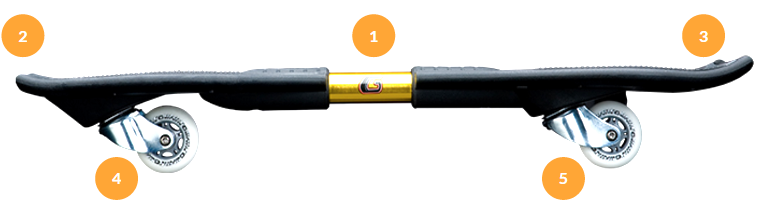
\includegraphics[width=\linewidth]{RipStikModel.png}
	\caption{Image depicting the 5 separate bodies of the RipStik}\label{fig:RipStikModel}
	\endminipage
\end{figure}  

Difficulties associated with accurately modeling the complex geometry of the RipStik led to simplifying assumptions being made for the shapes of the 5 separate bodies.
The front and back plates were treated as rectangular prisms while defining inertia tensors for the bodies, and the inertia tensors for the wheels were combined with the casters. 
Additionally, the casters were treated as skates to emulate the constrained motion of the casters while simplifying the overall system dynamics.
\par
The spring in the torsion rod was omitted since it is not a critical component of the RipStik and will add unnecessary complexity to the system in the form of kinetic energy.
Friction between the bodies of the RipStik was omitted, since it would be difficult to accurately model and does not have a significant impact on the general dynamics of the system.

\subsection{Coordinate Systems}

The initial focus for developing a mathematical model of the RipStik was placed on determining the number of degrees of freedom in the system. 
A coordinate system was defined, assumptions were made, and Euler angles were applied to said coordinate system so that all degrees of freedom could be explicitly defined.
\par
A body-fixed coordinate system for the RipStik was developed such that the origin was placed at the center of the torsion bar. The X-Y plane will be parallel with the RipStik Deck at rest with no torsion applied.
The +X direction points through the torsion bar towards the front plate, and the Y axis is defined perpendicular to the X axis. The Z axis is normal to the X-Y plane, with +Z pointing upwards. The +Y direction is defined based on the right hand rule.

With the coordinate system defined, Euler angles were implemented into the system to represent the roll ($\alpha$), pitch ($\psi$), and yaw ($\theta$).
\par
The roll angles ($\alpha$) describe the rotation of the deck platform about the X-axis. There will be two roll angles on the RipStik, the first on the front platform ($\alpha_{fp}$) and the second on the rear platform ($\alpha_{bp}$).
\par
The pitch angle ($\psi$) is the angle that the wheels make, offset by the caster angle ($\phi$). This represents a rotation about the Y axis. The wheels are completely unbounded in their ability to rotate, and can pivot through [0, 2$\pi$].
\par
The yaw angle ($\theta$) was represented by a moment taken around the Z-axis (right hand rule applied). There will be two yaw angles on the RipStik, the first on the front caster ($\theta_{fc}$), and the second on the back caster ($\theta_{bc}$).

The RipStik has ten degrees of freedom represented by [X, Y, Z, $\alpha$, $\psi$, $\theta$, $\alpha_{fp}$, $\alpha_{bp}$, $\theta_{fc}$, $\theta_{bc}$].

\subsubsection{Test Case - Caster Rotation}

In order to validate the selected coordinate system, a test case was conducted for RipStik. This was done by analyzing the behavior of the caster as it went through a full revolution (2$\pi$ radians).
The output for the X,Y, and Z positions were plotted as a function of the casters rotation as seen in Figure \ref{fig:CasterWheel2DTest}.

\begin{figure}[!htb]
	\centering
	\minipage{0.7\textwidth}
	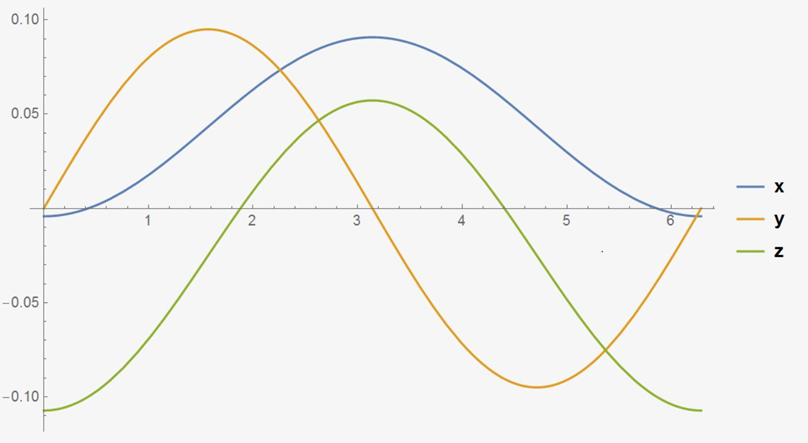
\includegraphics[width=\linewidth]{CasterWheel2DTest.png}
	\caption{The X ,Y, and Z positions of the caster were plotted as a function of the caster angle (in radians)}\label{fig:CasterWheel2DTest}
	\endminipage
\end{figure} 

With the two-dimensional plot completed, a three-dimensional plot was created to ensure that the casters obeyed the caster orientation that was previously defined, and can be seen in Figure \ref{fig:CasterWheel3DTest}.

\begin{figure}[!htb]
	\centering
	\minipage{0.7\textwidth}
	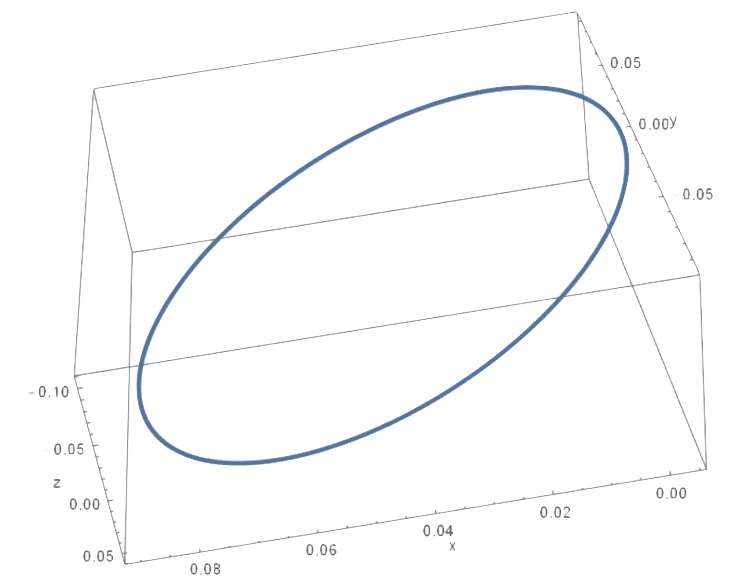
\includegraphics[width=\linewidth]{CasterWheel3DTest.png}
	\caption{The X ,Y, and Z positions of the caster were plotted as a function of the caster angle (in radians) on a three-dimensional plot}\label{fig:CasterWheel3DTest}
	\endminipage
\end{figure} 

\subsubsection{Model Implementation}

With the test case completed and verified, the coordinate system for the RipStik model was verified for each degree of freedom in the system. 
This was completed by taking applying the output from Mathematica into the ThreeJS based visualization tool.

\textbf{INCLUDE SCREENSHOT FROM ANIMATION?}
\subsubsection{Validation}

Each degree of freedom in the system behaved as expected. 
Therefore, the selected coordinate system was correct, and the equations of motion can be developed.

\subsection{Equations of Motion}

To develop the equations of motion for the RipStik, the Lagrangian needs to be clearly developed. Given Equation \ref{eq:Lagrange}, it is necessary to break down the components of kinetic and potential energies in the system.

The kinetic energy in the system is composed of translational and rotational components.
The Translational Kinetic Energy (TKE) is modeled in the following fashion:

\begin{equation}
\label{eq:TKE}
\text{TKE} = \frac{1}{2}{\text{m}}{\lvert \lvert {\dot{\text{r}}^2} \rvert \rvert}
\end{equation}

In Equation \ref{eq:TKE}, m represents the mass of the body and $\dot{r}$ represents the translational velocity of the body.
\par
The Rotational kinetic energy (RKE) is modeled in the following fashion:

\begin{equation}
\label{eq:RKE}
\text{RKE} = \frac{1}{2}({\text{I}}{\omega(t)})^T\omega(t)
\end{equation}

In Equation \ref{eq:RKE}, I represents the inertia tensor of the body, and $\omega(t)$ represents the angular velocity of the body.

Finding the angular velocity for the body requires the following process. First, $\hat{\omega(t)}$ is solved for using Equation \ref{eq:omegahat}.

\begin{equation}
\label{eq:omegahat}
\hat{\omega}(t)=R^T(t)\dot{R(t)}
\end{equation}

Equation \ref{eq:omegahat} generates a 3x3 skew-symmetric matrix. The angular velocity is then a column vector composed of 3 elements from $\hat{\omega}(t)$, seen in Equation \ref{eq:omega}.

\begin{equation}
\label{eq:omega}
\omega(t)=\begin{bmatrix}
\hat{\omega}(t)[3,2] \\
\hat{\omega}(t)[1,3] \\
\hat{\omega}(t)[2,1]\\
\end{bmatrix}
\end{equation}

The potential energy in the system is composed of only Gravitational Potential Energy (GPE). This is modelled by Equation \ref{eq:GPE}.

\begin{equation}
\label{eq:GPE}
\text{GPE} = {\text{m}}{\text{g}}{\text{h}}
\end{equation}

In Equation \ref{eq:GPE}, m represents the mass of the body and h represents the height of the body relative to the ground plane.

With the kinetic and potential energies explicitly defined, the Lagrangian can be written as follows:

\begin{equation}
L= \frac{1}{2}{\text{m}}{\lvert \lvert {\dot{\text{r}}^2} \rvert \rvert} + \frac{1}{2}({\text{I}}{\omega(t)})^T\omega(t) - {\text{m}}{\text{g}}{\text{h}}
\end{equation}

The explicit Lagrangian can then be applied to the Euler-Lagrange equations do develop the ten unconstrained equations of motion for each degree of freedom using Equation \ref{eq:UEOM}.

\subsubsection{Test Case - Uncontrolled Inverted Pendulum}\label{sec:testcaseip}

The equations of motion were validated using an unconstrained system. A pendulum  attached to a moving cart with an initial position pointing upwards was modeled using Lagrangian mechanics. 
The mass of the cart is defined as $m_{1}$ and the mass of the pendulum is defined as $m_{2}$. 
The set up of the coordinate system can be seen in figure \ref{fig:pendulumcart}.

\begin{figure}[!htb]
	\centering
	\minipage{0.5\textwidth}
	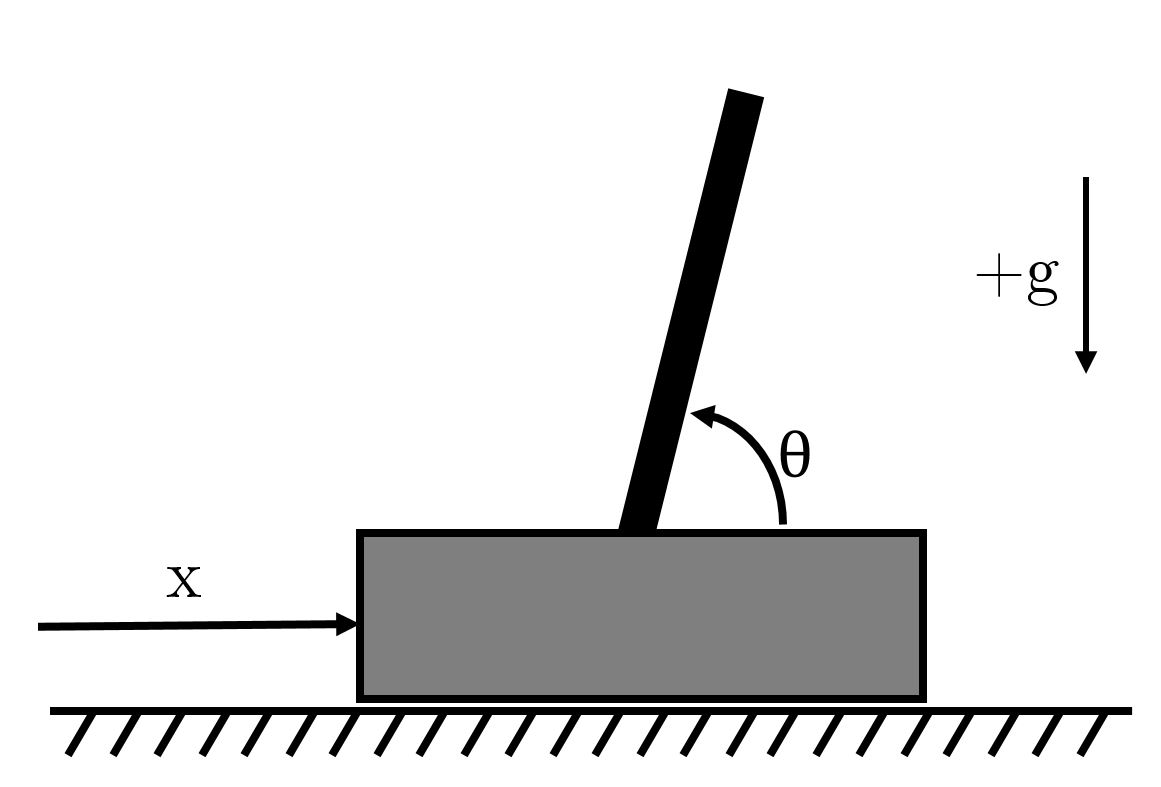
\includegraphics[width=\linewidth]{pendulumcart}
	\caption{Model set-up for the pendulum cart example}\label{fig:pendulumcart}
	\endminipage
\end{figure} 

The Lagrangian for the system is seen in Equation \ref{eq:CartLagrange}.

\begin{equation}
\label{eq:CartLagrange}
L = \frac{1}{2}m_{1}X'(t)^2+\frac{1}{2}m_{2}(2gL\sin\theta(t)+2L^2\theta'(t)^2-2L\sin\theta(t)\theta'(t)X'(t)+X'(t)^2) 
\end{equation}

With the Lagrangian developed, the equations of motion were solved for the two degrees of freedom (X(t), $\theta(t)$):

\begin{equation}
Lm_{2}\cos\theta(t)\theta'(t)^2+Lm_{2}\sin\theta(t)\theta''(t)-(m_{1}+m_{2})X''(t) = 0
\end{equation}

\begin{equation}
Lm_{2}(g\cos\theta(t)-2L\theta''(t)+\sin\theta(t)X''(t)) = 0
\end{equation}

With these equations of motion, it was confirmed that the pendulum reacted as expected when the cart moved positions.

\subsubsection{Model Implementation}

With the test case complete, the equations of motion were tested on the RipStik model. A Z coordinate in the center of the torsion rod of the RipStik was fixed.
An initial roll angle of 45 degrees was applied to the front plate ($\alpha_{fp}$), and an initial roll angle of -45 degrees was applied to the back plate ($\alpha_{bp}$). 

\subsubsection{Validation}

When the model implementation was tested with the conditions specified previously, the RipStik behaved as expected. 
The front and back plated experienced an oscillating motion between 45 and -45 degrees, with the casters rotating between 45 and -45 degrees. 
Plots for roll of the front plate ($\alpha_{fp}$), roll of the back plate ($\alpha_{bp}$), yaw of the front caster ($\theta_{fc}$), and yaw of the back caster ($\theta_{bc}$) were plotted to ensure that the motion of the Ripstik aligned with the expected behaviour.

\begin{figure}[!htb]
	\centering
	\minipage{0.4\textwidth}
	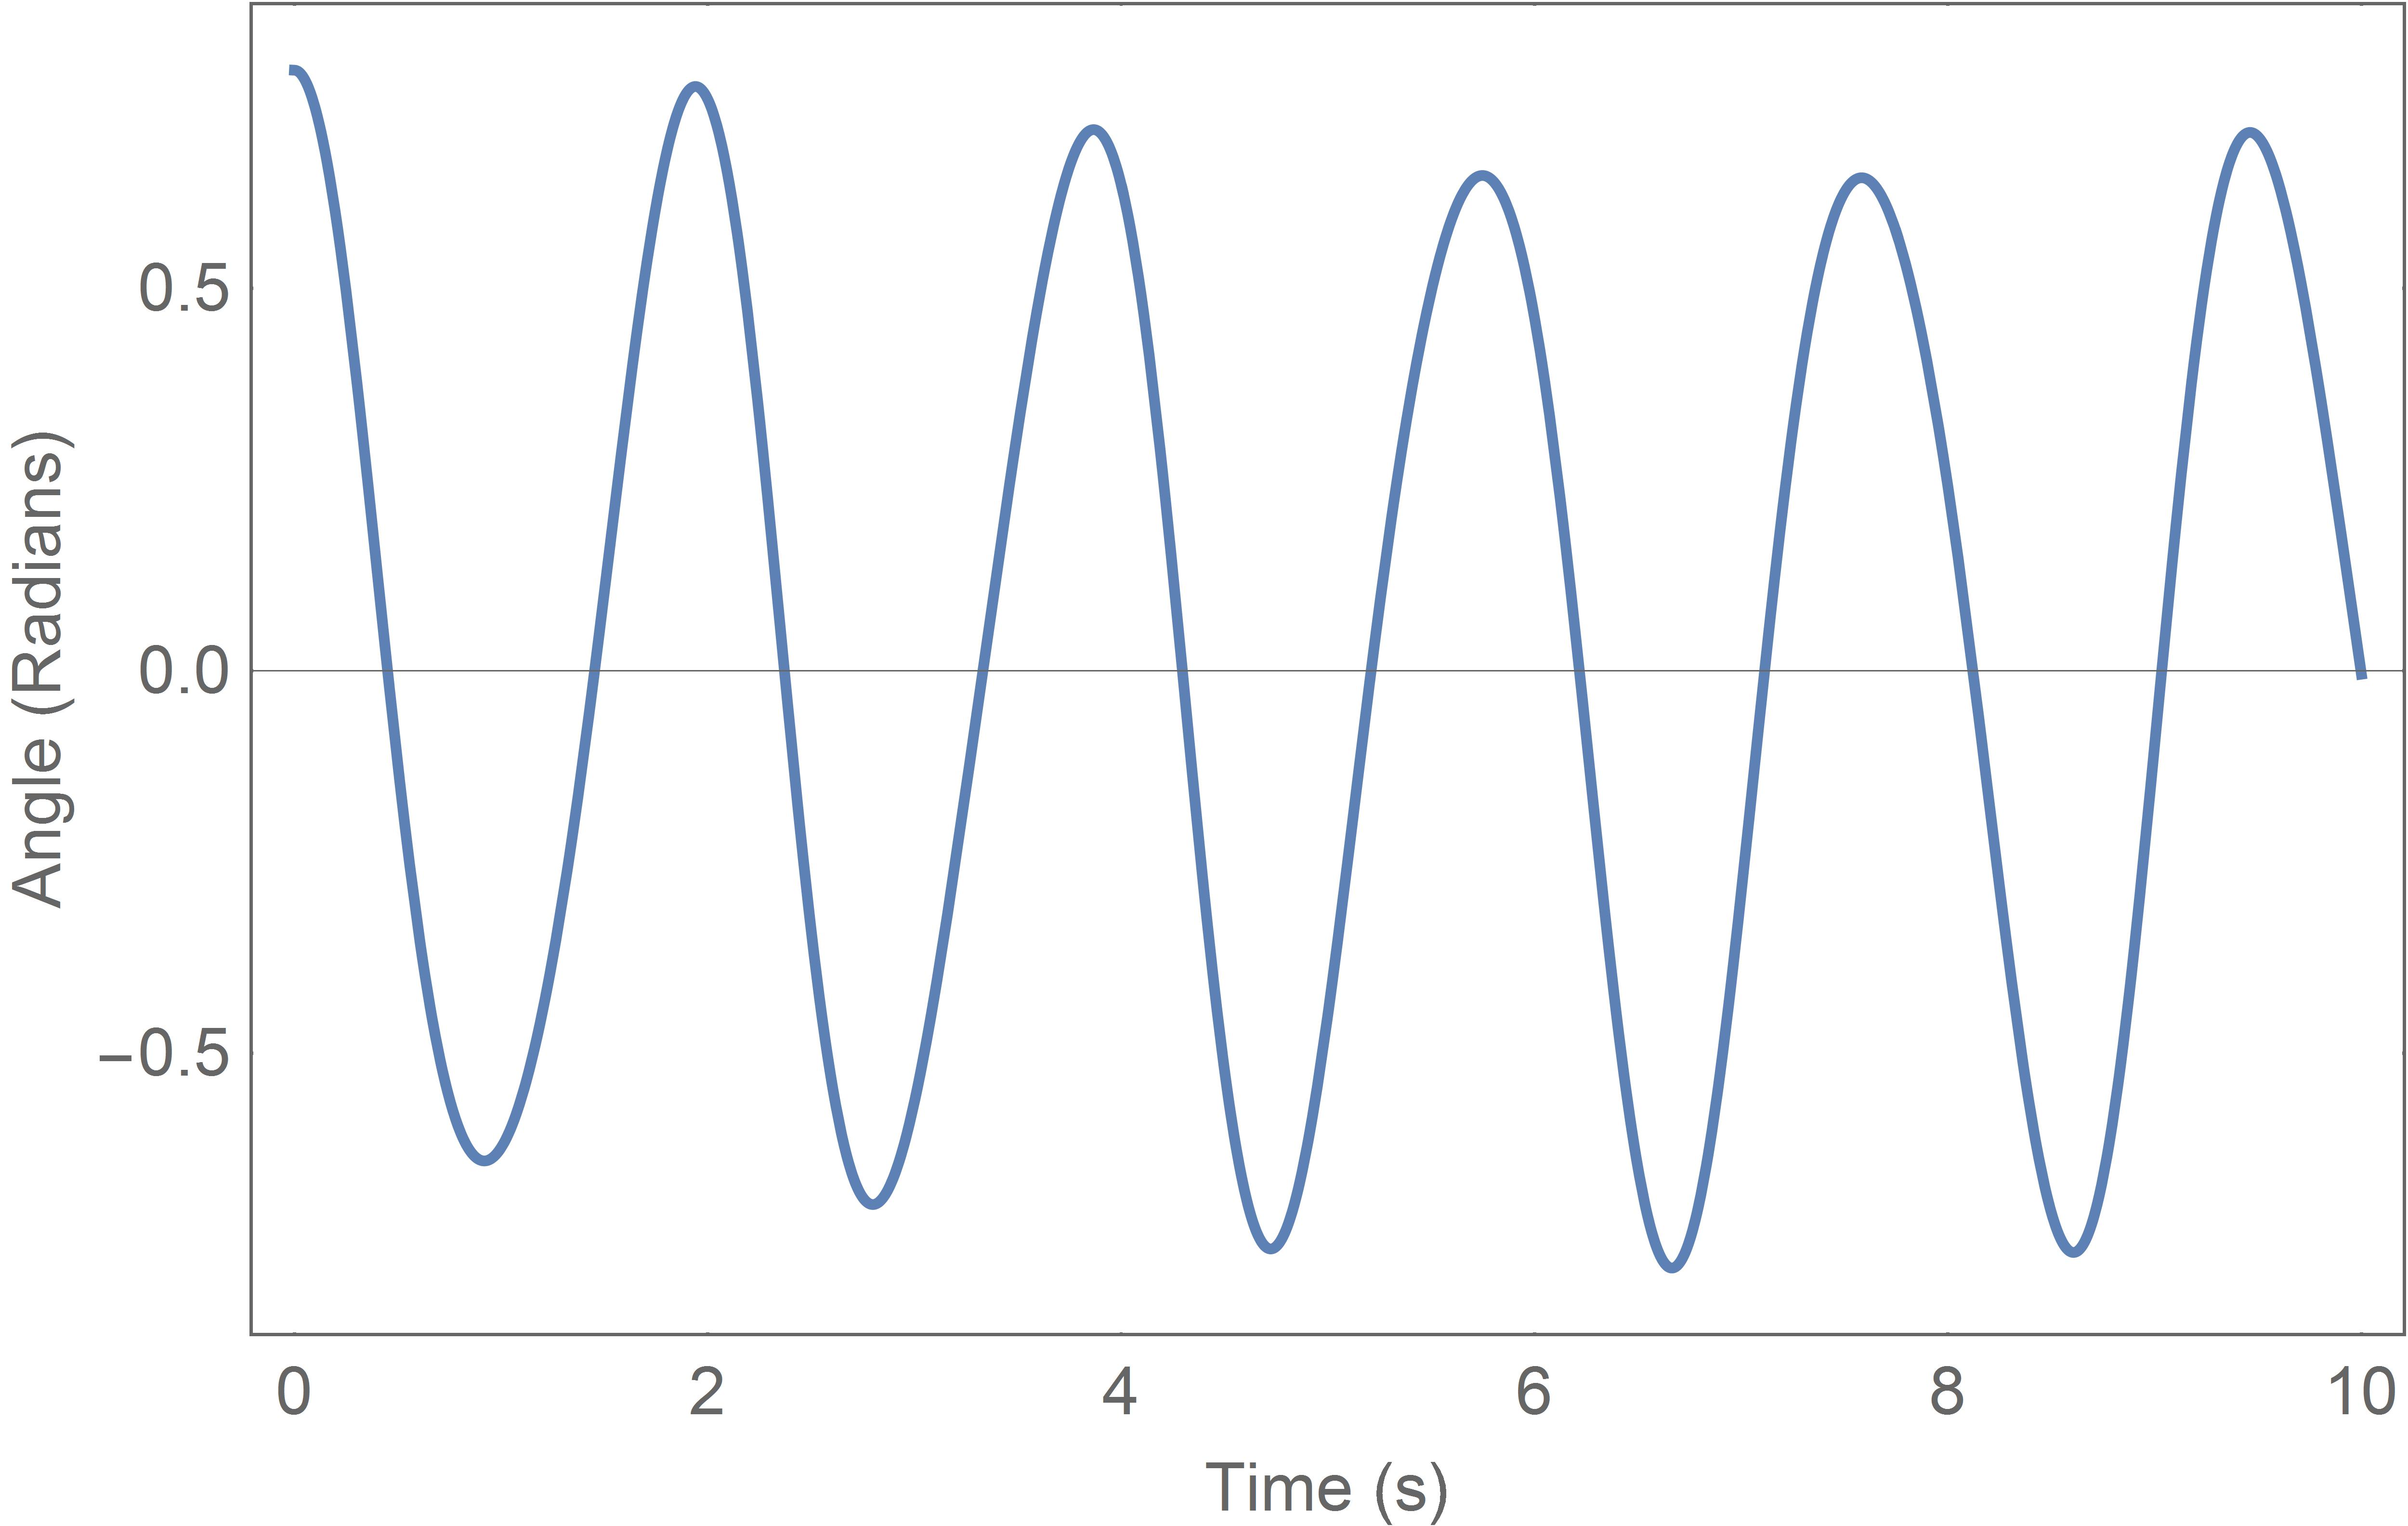
\includegraphics[width=\linewidth]{alphafp}
	\endminipage\hspace{1em}%
	\minipage{0.4\textwidth}
	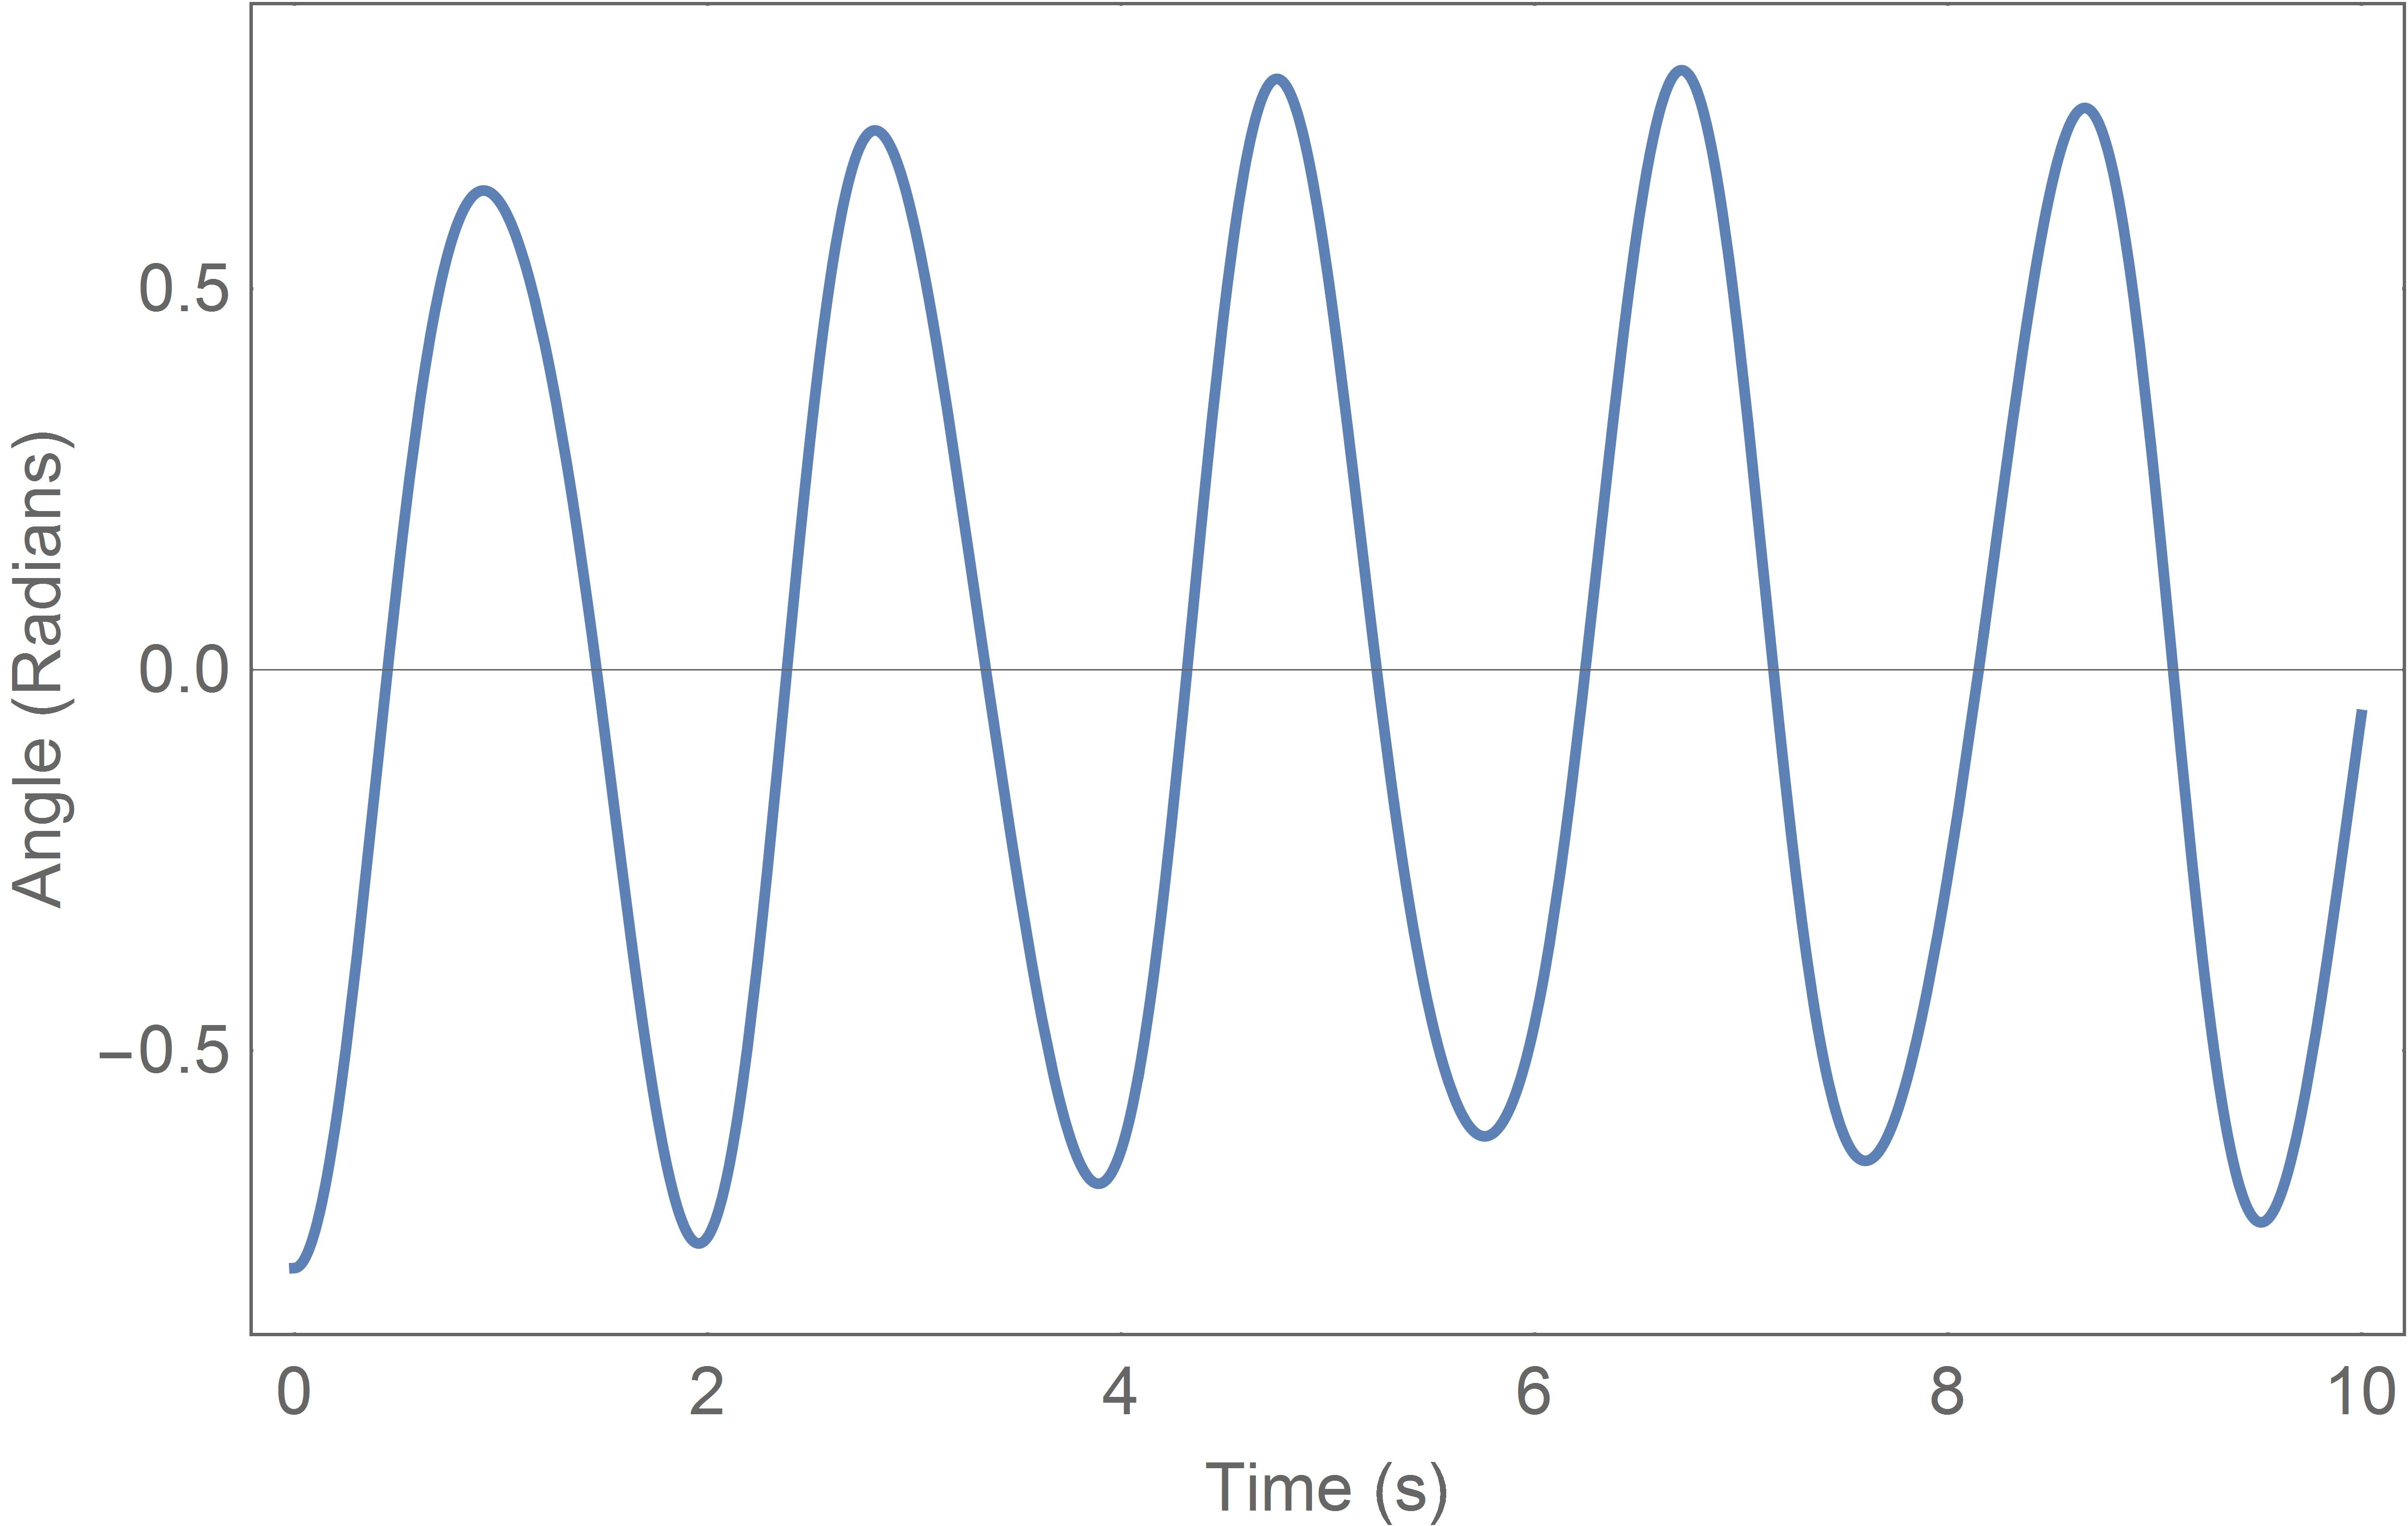
\includegraphics[width=\linewidth]{alphabp}
	\endminipage
	\caption{Roll of front plate ($\alpha_{fp}$) and back plate ($\alpha_{bp}$)}
	\label{fig:plates}
\end{figure}

\begin{figure}[!htb]
	\centering
	\minipage{0.4\textwidth}
	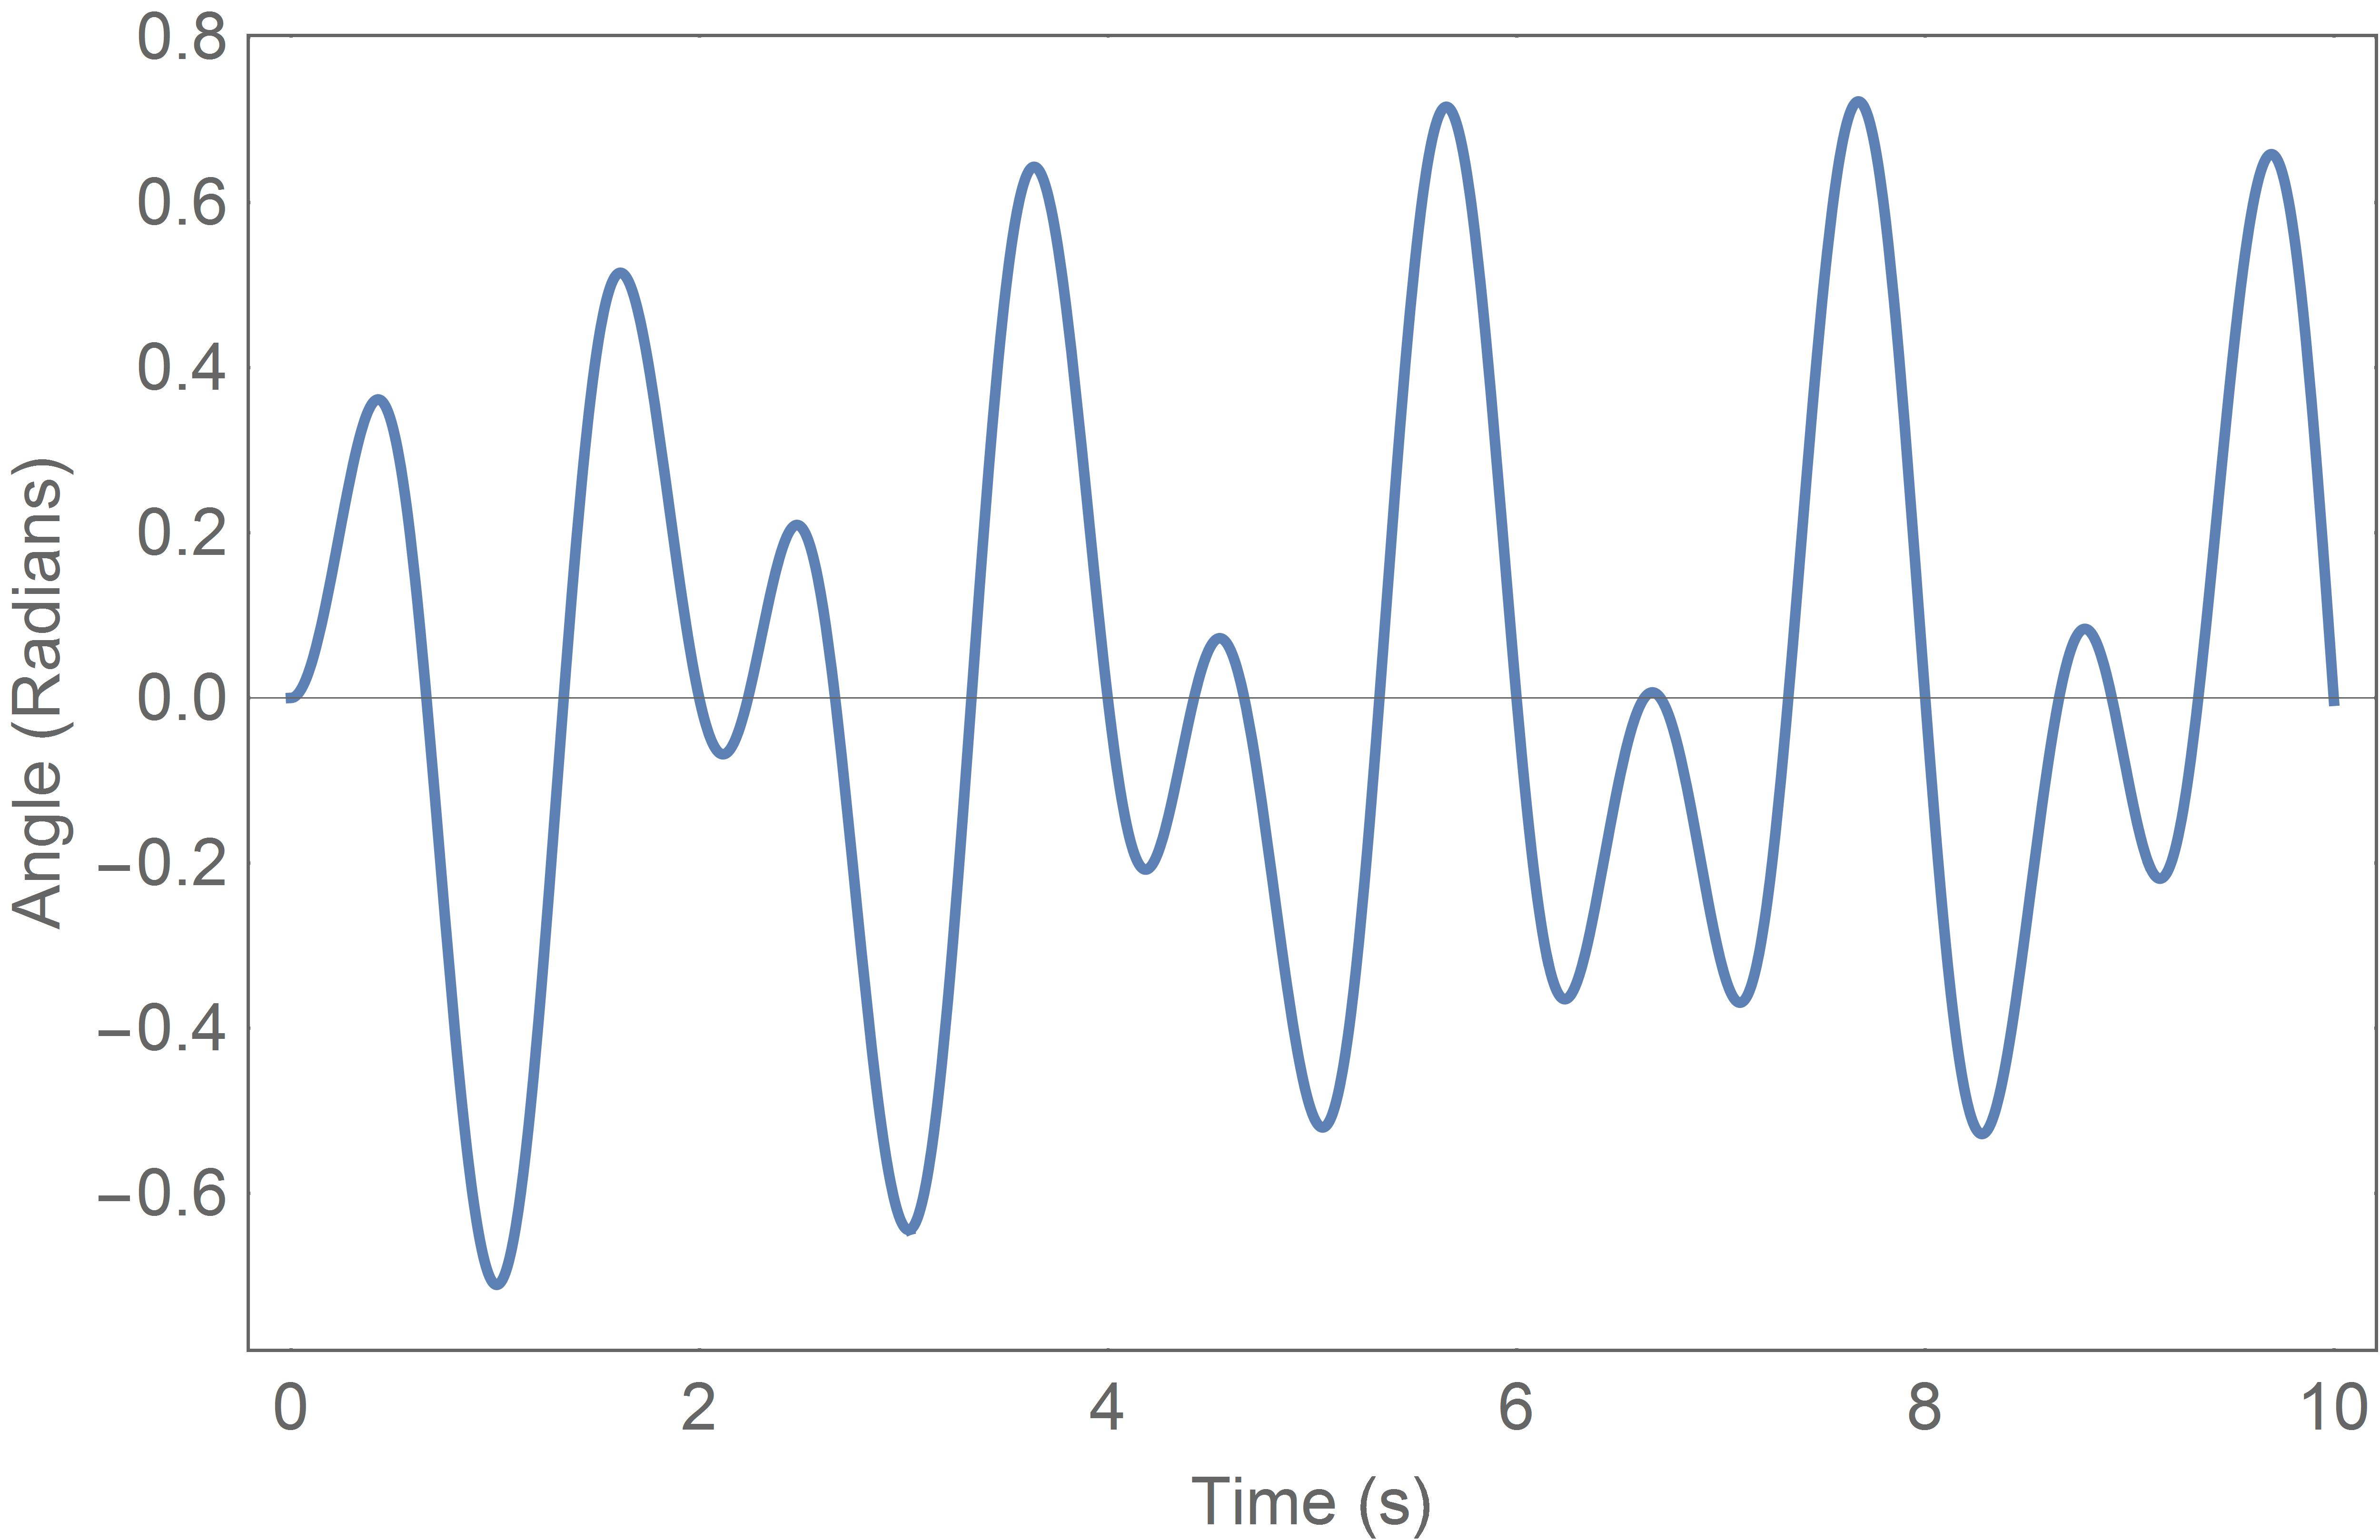
\includegraphics[width=\linewidth]{thetafc}
	\endminipage\hspace{1em}%
	\minipage{0.4\textwidth}
	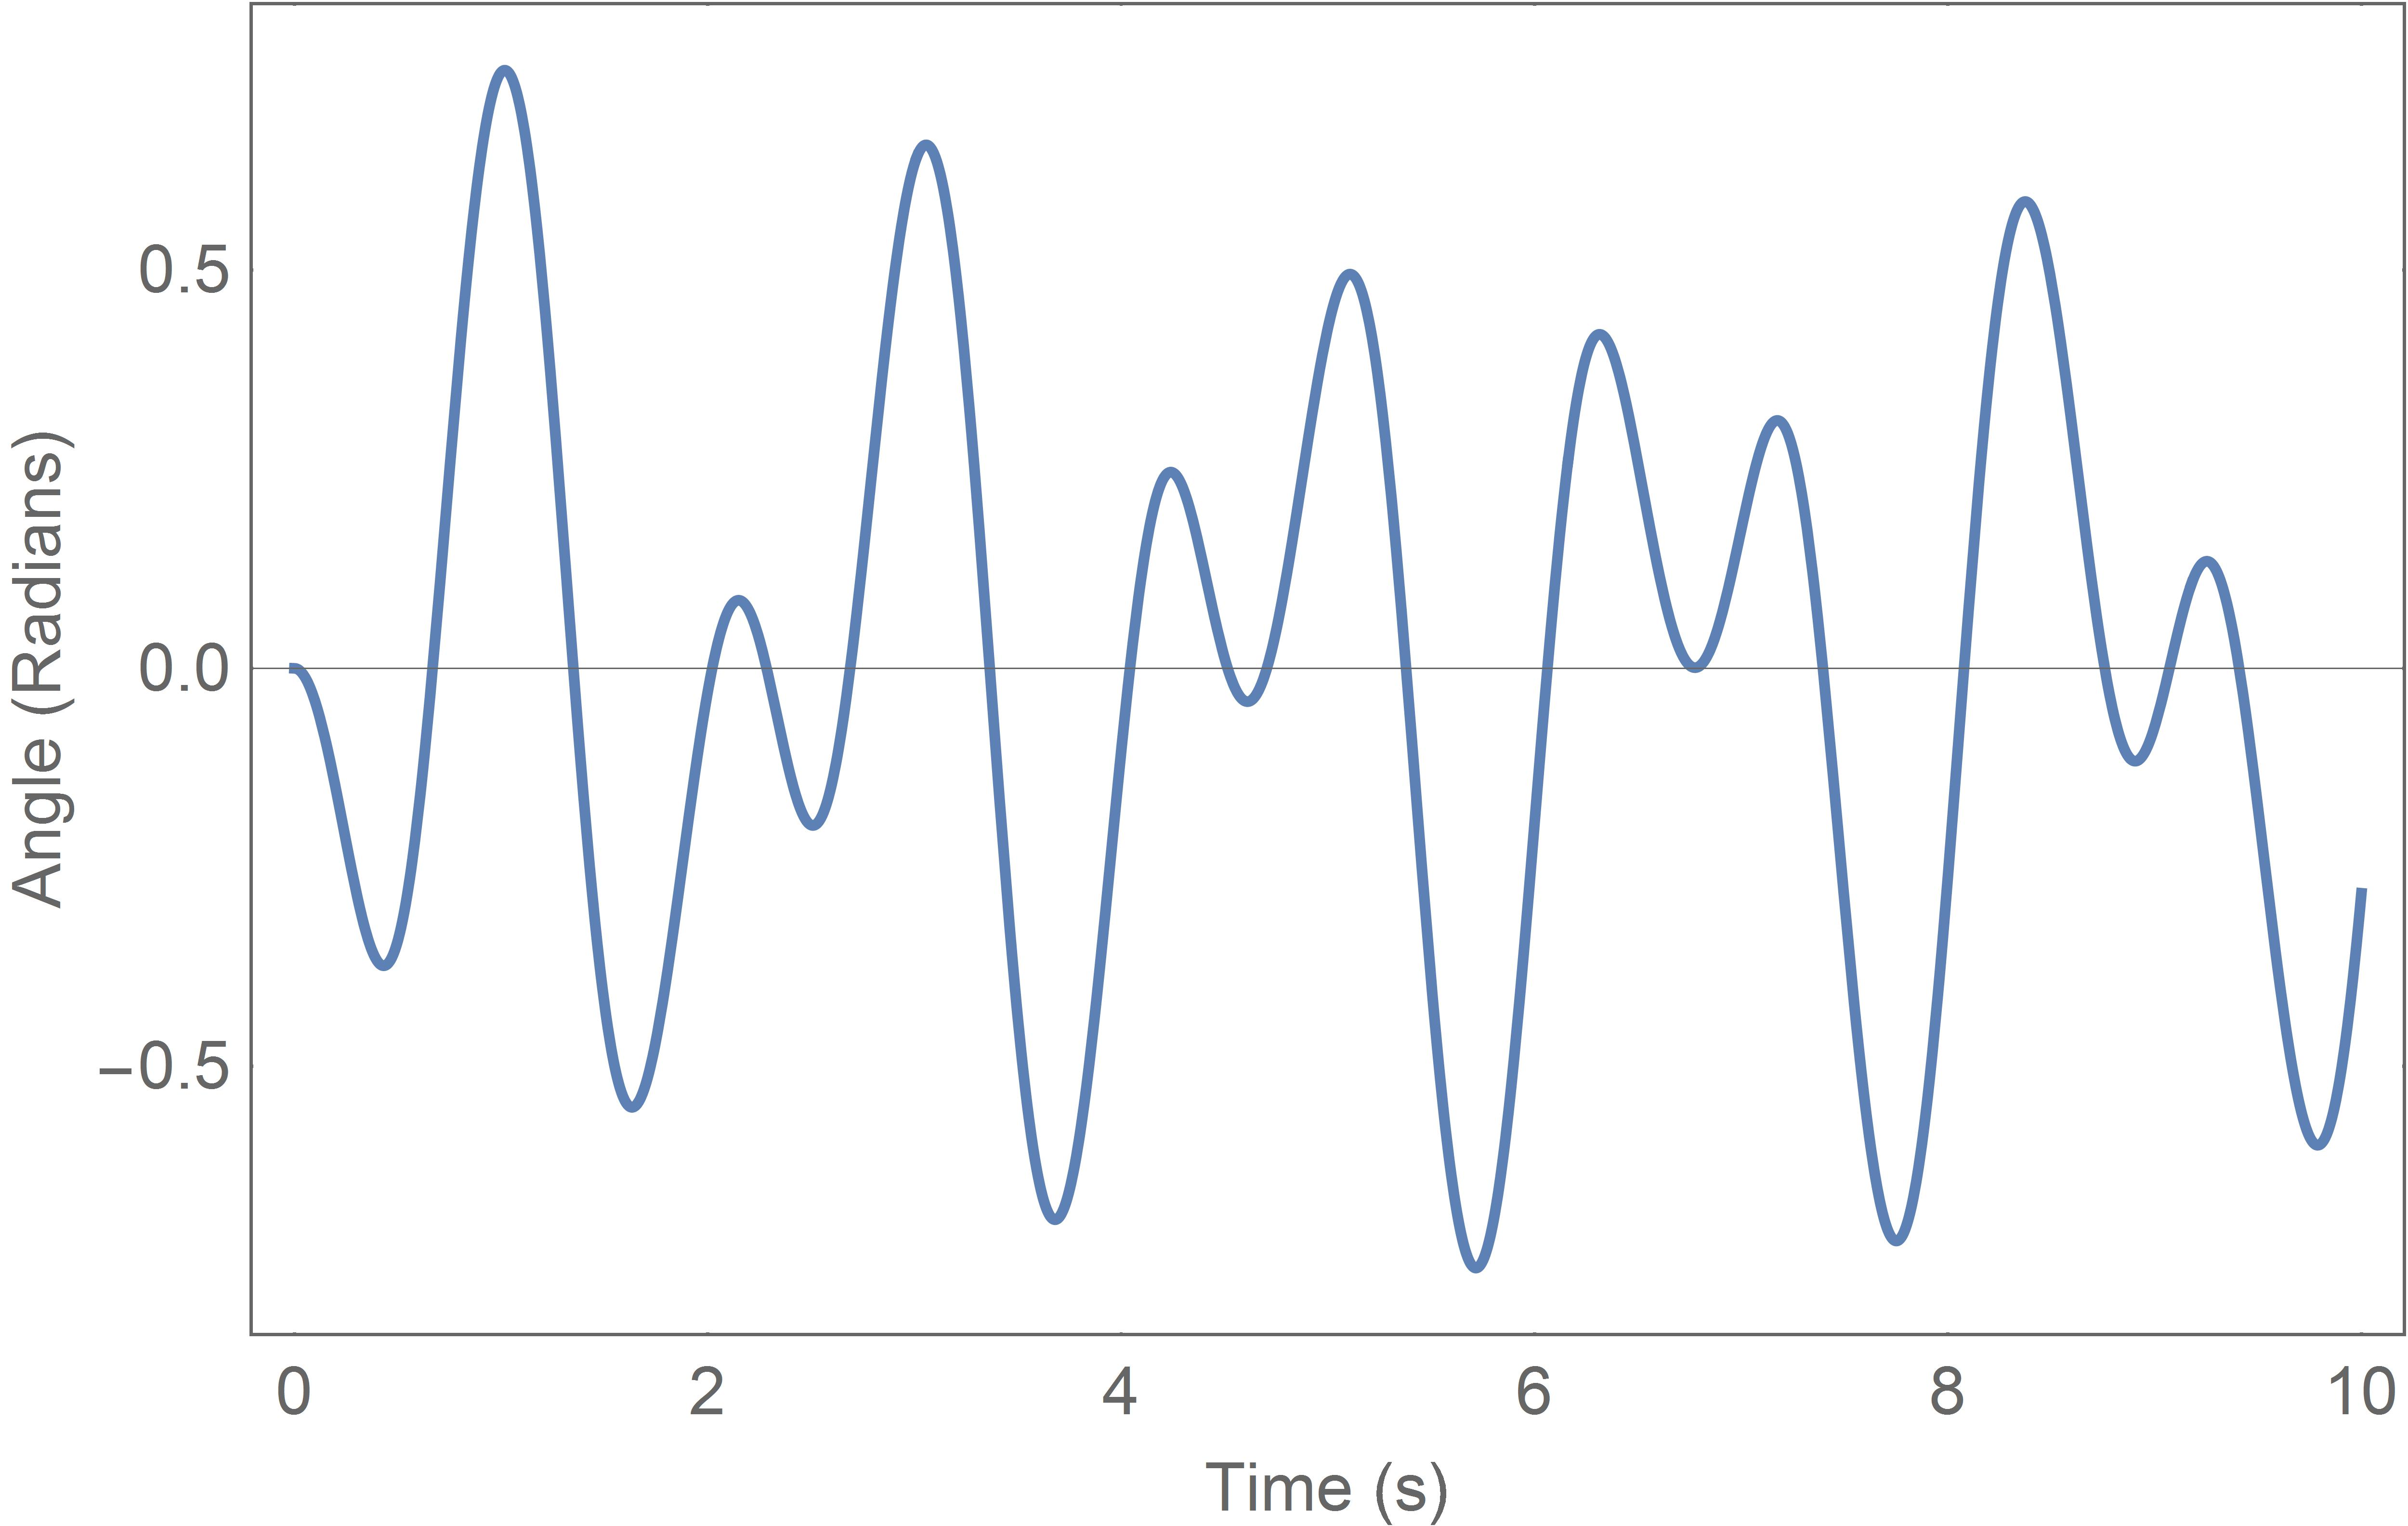
\includegraphics[width=\linewidth]{thetabc}
	\endminipage
	\caption{Yaw of front caster ($\theta_{fc}$) and back caster ($\theta_{bc}$)}
	\label{fig:casters}
\end{figure}

Since the plates and casters both experienced oscillations approximately between 45 and -45 degrees, it can be confirmed that the equations of motion for the RipStick were accurate.

An accurate visualization of the Ripstik was produced to model the motion and the two extreme positions of the RipStik can be seen in figure \ref{fig:RipStikModel1}.

\begin{figure}[!htb]
	\centering
	\minipage{0.4\textwidth}
	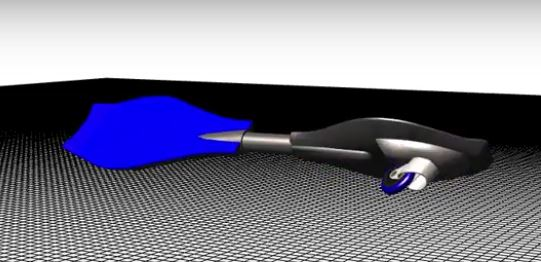
\includegraphics[width=\linewidth]{oneswing}
	\endminipage\hspace{1em}%
	\minipage{0.42\textwidth}
	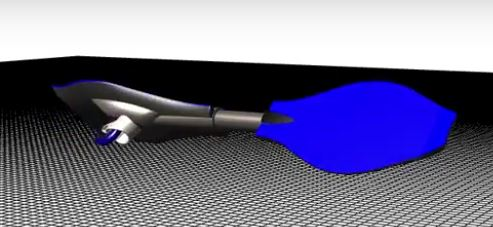
\includegraphics[width=\linewidth]{twoswing}
	\endminipage
	\caption{Two extreme positions of the RipStik motion}
	\label{fig:RipStikModel1}
\end{figure}

\subsection{Nonholonomic Constraints}

With the unconstrained equations of motion validated, nonholonomic constraints were implemented into the system. 
The constraints were defined such that the wheels could not slide laterally or lift off the ground. 
This represented a total of four constraint forces which were implemented using Lagrange multipliers.
Three different methods were explored when trying to solve for the nonholonomic constraints: symbolically inverting the matrices, representing the constraints as a system of linear equations $(Ax=B)$, and numeric integration.

\paragraph{Symbolic Matrix Inversion}\mbox{}\\
The initial method explored involved symbolically inverting matrices in Mathematica. First, the acceleration terms in the equations of motion were isolated for, which could then be substituted into the derivatives of the nonholonomic constraint equations, seen in Equation \ref{eq:SMI}.

\begin{equation}
\label{eq:SMI}
\Omega \ddot{q} = -\Omega G_{jk}^{-1}\Gamma_{jkl} \dot{q}^k\dot{q}^l + \Omega G_{jk}^{-1} \Omega ^T \lambda
\end{equation}

This is an intuitive approach from a linear algebra perspective; however, it is computationally impossible on large scale systems. 
When trying to solve for the acceleration terms, the computer's RAM completely fills and Mathematica is forced to abandon the calculation.

%%%%%%%%%%%%%%%%%%%%%%%%%%%%%%%%%%%%%%%%%%%%%%%%%%%
%%%%%%
%%%%%% MORE SPECIFIC ABOUT WHY RAM FILLS IE DETERMINANTS. Double check equation, the coeffs look a little fucky?
%%%%%%
%%%%%%%%%%%%%%%%%%%%%%%%%%%%%%%%%%%%%%%%%%%%%%%%%%%
\paragraph{System of Linear Equations $(Ax=B)$}\mbox{}\\
The next method attempted required taking the matrix inversion and representing it as a system of linear equations of the form Ax=b. 
In this equation, A is a square matrix and b is a column vector.
This allows Mathematics more flexibility to internally choose from three different approaches for isolating the desired results, using Laplace cofactor expansion, Bareiss method of division-free row reduction, and standard row reduction for computing determinants \cite{linearsolve}.
Bareiss method of division-free row reduction allows for the computation of determinants without introducting fractions \cite{bareiss}.
\par
At this point, all symbolic constants were replaced with with measured values to further simplify computations.
Using this method, the accelerations were solved in the equations of motion, but trying to find the lagrange multipliers in the second system exceeded computation times.

\paragraph{Numeric Integration}\mbox{}\\
The final method analyzed involved solving the system numerically.
Using this method, Equations \ref{eq:CFE} and \ref{eq:CV} can remain in their initial form.
Numeric integration functions can then be applied to approximate the result of the system of differential equations and ultimately produce output from the model.
A drawback associated with this method is that it can be a difficult process requiring careful tuning of numerical integrators and ultimately does not give explicit equations for the constraints.

\subsubsection{Test Case - Rolling Wheel}\label{sec:testcaserw}

Prior to implementing the three methods in the RipStik system, a simple model of a rolling wheel was used to validate the different approaches. For nonholonomic constraints, a code was developed and tested on the simple example of a wheel that rolls without slipping.
No slip constraints are considered to be nonholonomic, and the output can be easily compared to published results.
The configuration space for the rolling wheel consists of [X(t), Y(t), $\theta(t)$, $\phi(t)$].
The Lagragian for the system is seen in Equation \ref{eq:rollingdicks}.

\begin{equation}
\label{eq:rollingdicks}
L=\frac{1}{2}(mX'(t)^2+mY'(t)^2+Jroll\theta'(t)^2+Jspin\phi'(t)^2)
\end{equation}

With the Lagrangian developed, it was then applied to the Euler-Lagrange equations to provide the equations of motion, seen in equations \ref{eq:Xroll}, \ref{eq:Yroll}, \ref{eq:thetaroll}, and \ref{eq:phiroll}.

\begin{equation}
\label{eq:Xroll}
-mX''(t)=0
\end{equation}

\begin{equation}
\label{eq:Yroll}
-mY''(t)=0
\end{equation}

\begin{equation}
\label{eq:thetaroll}
-Jroll\theta''(t)=0
\end{equation}

\begin{equation}
\label{eq:phiroll}
-Jspin\phi''(t)=0
\end{equation}

\subsubsection{Model Implementation}

While all three approaches worked perfectly on the rolling wheel, they did not scale as desired to the much larger RipStik system.
The complexity of the system led to computations that exceeded the computer's abilities for the symbolic matrix inversion and system of linear equations.
Ultimately, numeric integration was selected to produce output.

\subsubsection{Numeric Integration}

Numeric Integration allows for the approximate computation of an integral using numerical methods \cite{WolframNumeric}.
When applying numeric integration to a differential system, stiffness is often a by-product.
The concept of stiffness is not well understood, but can generally be attributed to quick changing dynamics in a system \cite{StiffSystem}.
\par
To help develop some intuition on how stiff systems work, an example can be seen in Figure \ref{fig:stiffsystem}.

\begin{figure}[!htb]
	\centering
	\minipage{0.7\textwidth}
	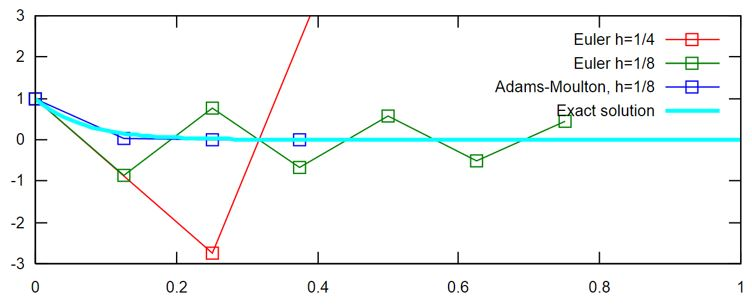
\includegraphics[width=\linewidth]{stiffsystem.JPG}
	\caption{Using numeric integration methods to approximate the exact solution to a differential equation}\label{fig:stiffsystem}
	\endminipage
\end{figure}
Figure \ref{fig:stiffsystem} shows the exact output from a simple differential equation in light blue. 
When numeric integration is attempted using Euler's method and a step size of 1/4, the approximation oscillates and completely overshoots the exact method as seen in red. 
When a step size of 1/8 is selected, there are still oscillations, but they are in a reasonable range around the exact solution as seen in green. 
When adams-Moulton method is used with a step size of 1/8, the oscillations are essesntially negligible and the approximation is almost equal to the exact solution.


\par
When a system has quickly changing dynamics, numeric integration will require increasingly small step sizes to approximate a solution without instability \cite{StiffSystem}. 
This adds computational complexity that ofteen exceeds modern technological capabilities. 
To try and reduce this computational complexity, four different numerical methods were selected to evaluate stiff DAE systems.

The QR Decomposition method decomposes the Jacobian of the derivative, breaking down the core system into two smaller systems at each iteration point \cite{Methods}.
This is represented by the following equation:

\begin{equation}
\label{eq:QR}
A = QR
\end{equation}

In Equation \ref{eq:QR}, A is any real square matrix, Q is an orthogonal matrix, and R is an upper triangular matrix \cite{Methods}.

The Collocation method linearizes the implicit DAE to m points in time, generating a system of linear equations which can be solved iteratively using Newton's Method \cite{Methods}.
The Implicit Differential-Algebraic Method uses Backward Differential Formulas (BDF) to implicity solve the DAE for derivatives to use an ODE solver \cite{Methods}. 
The BDF approximates the derivative of the function using information from previous time steps \cite{Methods}.
The BLT Method puts the system into block lower triangular form and solves subsets of the system iteratively \cite{Methods}.

While numeric integration produced results for the RipStik model, it brought its own set of challenges in the form of system stiffness.
For the RipStik, the frictionless linkages cause quick changes in the exact solution that is being approximated. 
When Mathematica attempts to numerically approximate this, it selects increasingly small step sizes to replicate these quick motions without oscillation. 
However, these increasingly small step sizes slow down the computation until Mathematica eventually abandons the attempt at numerically integrating over the chosen time interval.

\paragraph{Evaluation}\mbox{}\\
As previously discussed, four methods for numerically integrating stiff DAE systems were analyzed. 
QR decomposition, Collocation, IDA, and BLT methods were evaluated based on three criteria:
\begin{itemize}
\item The computation time was evaluated based on how long it would take for output to be generated (in seconds)
\item The duration of output was evaluated based on the length of the output computed (in seconds)
\item The reconfigurability of each method was evaluated qualitatively based on the number of tunable parameters that could be used to generate a greater length of output
\end{itemize}
A comparison of the results can be seen in Table \ref{table:evaluation}.

\begin{table}[ht]
	\caption{Numeric Integration Method Evaluation}
	\centering
	\def\arraystretch{1.3}
	\begin{tabular}{|c| c| c| c| c|}
		\hline\hline
		& QR Decomposition & \begin{tabular}{@{}c@{}}Collocation \\ Method\end{tabular} & IDA Method & BLT Method \\ 
		\hline
		Computation Time (s) & 1.2 & 26.4 & 1.2 & 1.2\\
		\hline
		Output Duration (s) & 0.6 & 5.8 & 0.6 & 0.6\\
		\hline
		Reconfigurability & Poor & Excellent & Good & Poor\\ [0.1ex]
		\hline
	\end{tabular}
	\label{table:evaluation}
\end{table}
From the results in table \ref{table:evaluation}, it is clear that there is a definitive tradeoff between computation time and length of output.
The Collocation method was able to produce output 9.7 times longer than all other methods, at a cost of 22 times longer computation.  
The gain in length of output was weighted far greater than the length of computation time, since the lengthened computation time was still feasible.

\subsubsection{Validation}

Using the Collocation integration method, 5.8 seconds of output for the falling RipStik was plotted for each degree of freedom in the system. 
As the RipStik fell, it eventually exceeded the range of validity for the Euler angles. 
This led to the RipStiks motion behaving eratically. 
As a result, only the first 1.4 seconds of the falling RipStik was plotted.

\begin{figure}[!htb]
	\centering
	\minipage{0.4\textwidth}
	\includegraphics[width=\linewidth]{fallz}
	\endminipage\hspace{1em}%
	\caption{The Z-position of the Ripstik as it falls}\label{fig:fallglobal}
\end{figure}

\begin{figure}[!htb]
	\centering
	\minipage{0.4\textwidth}
	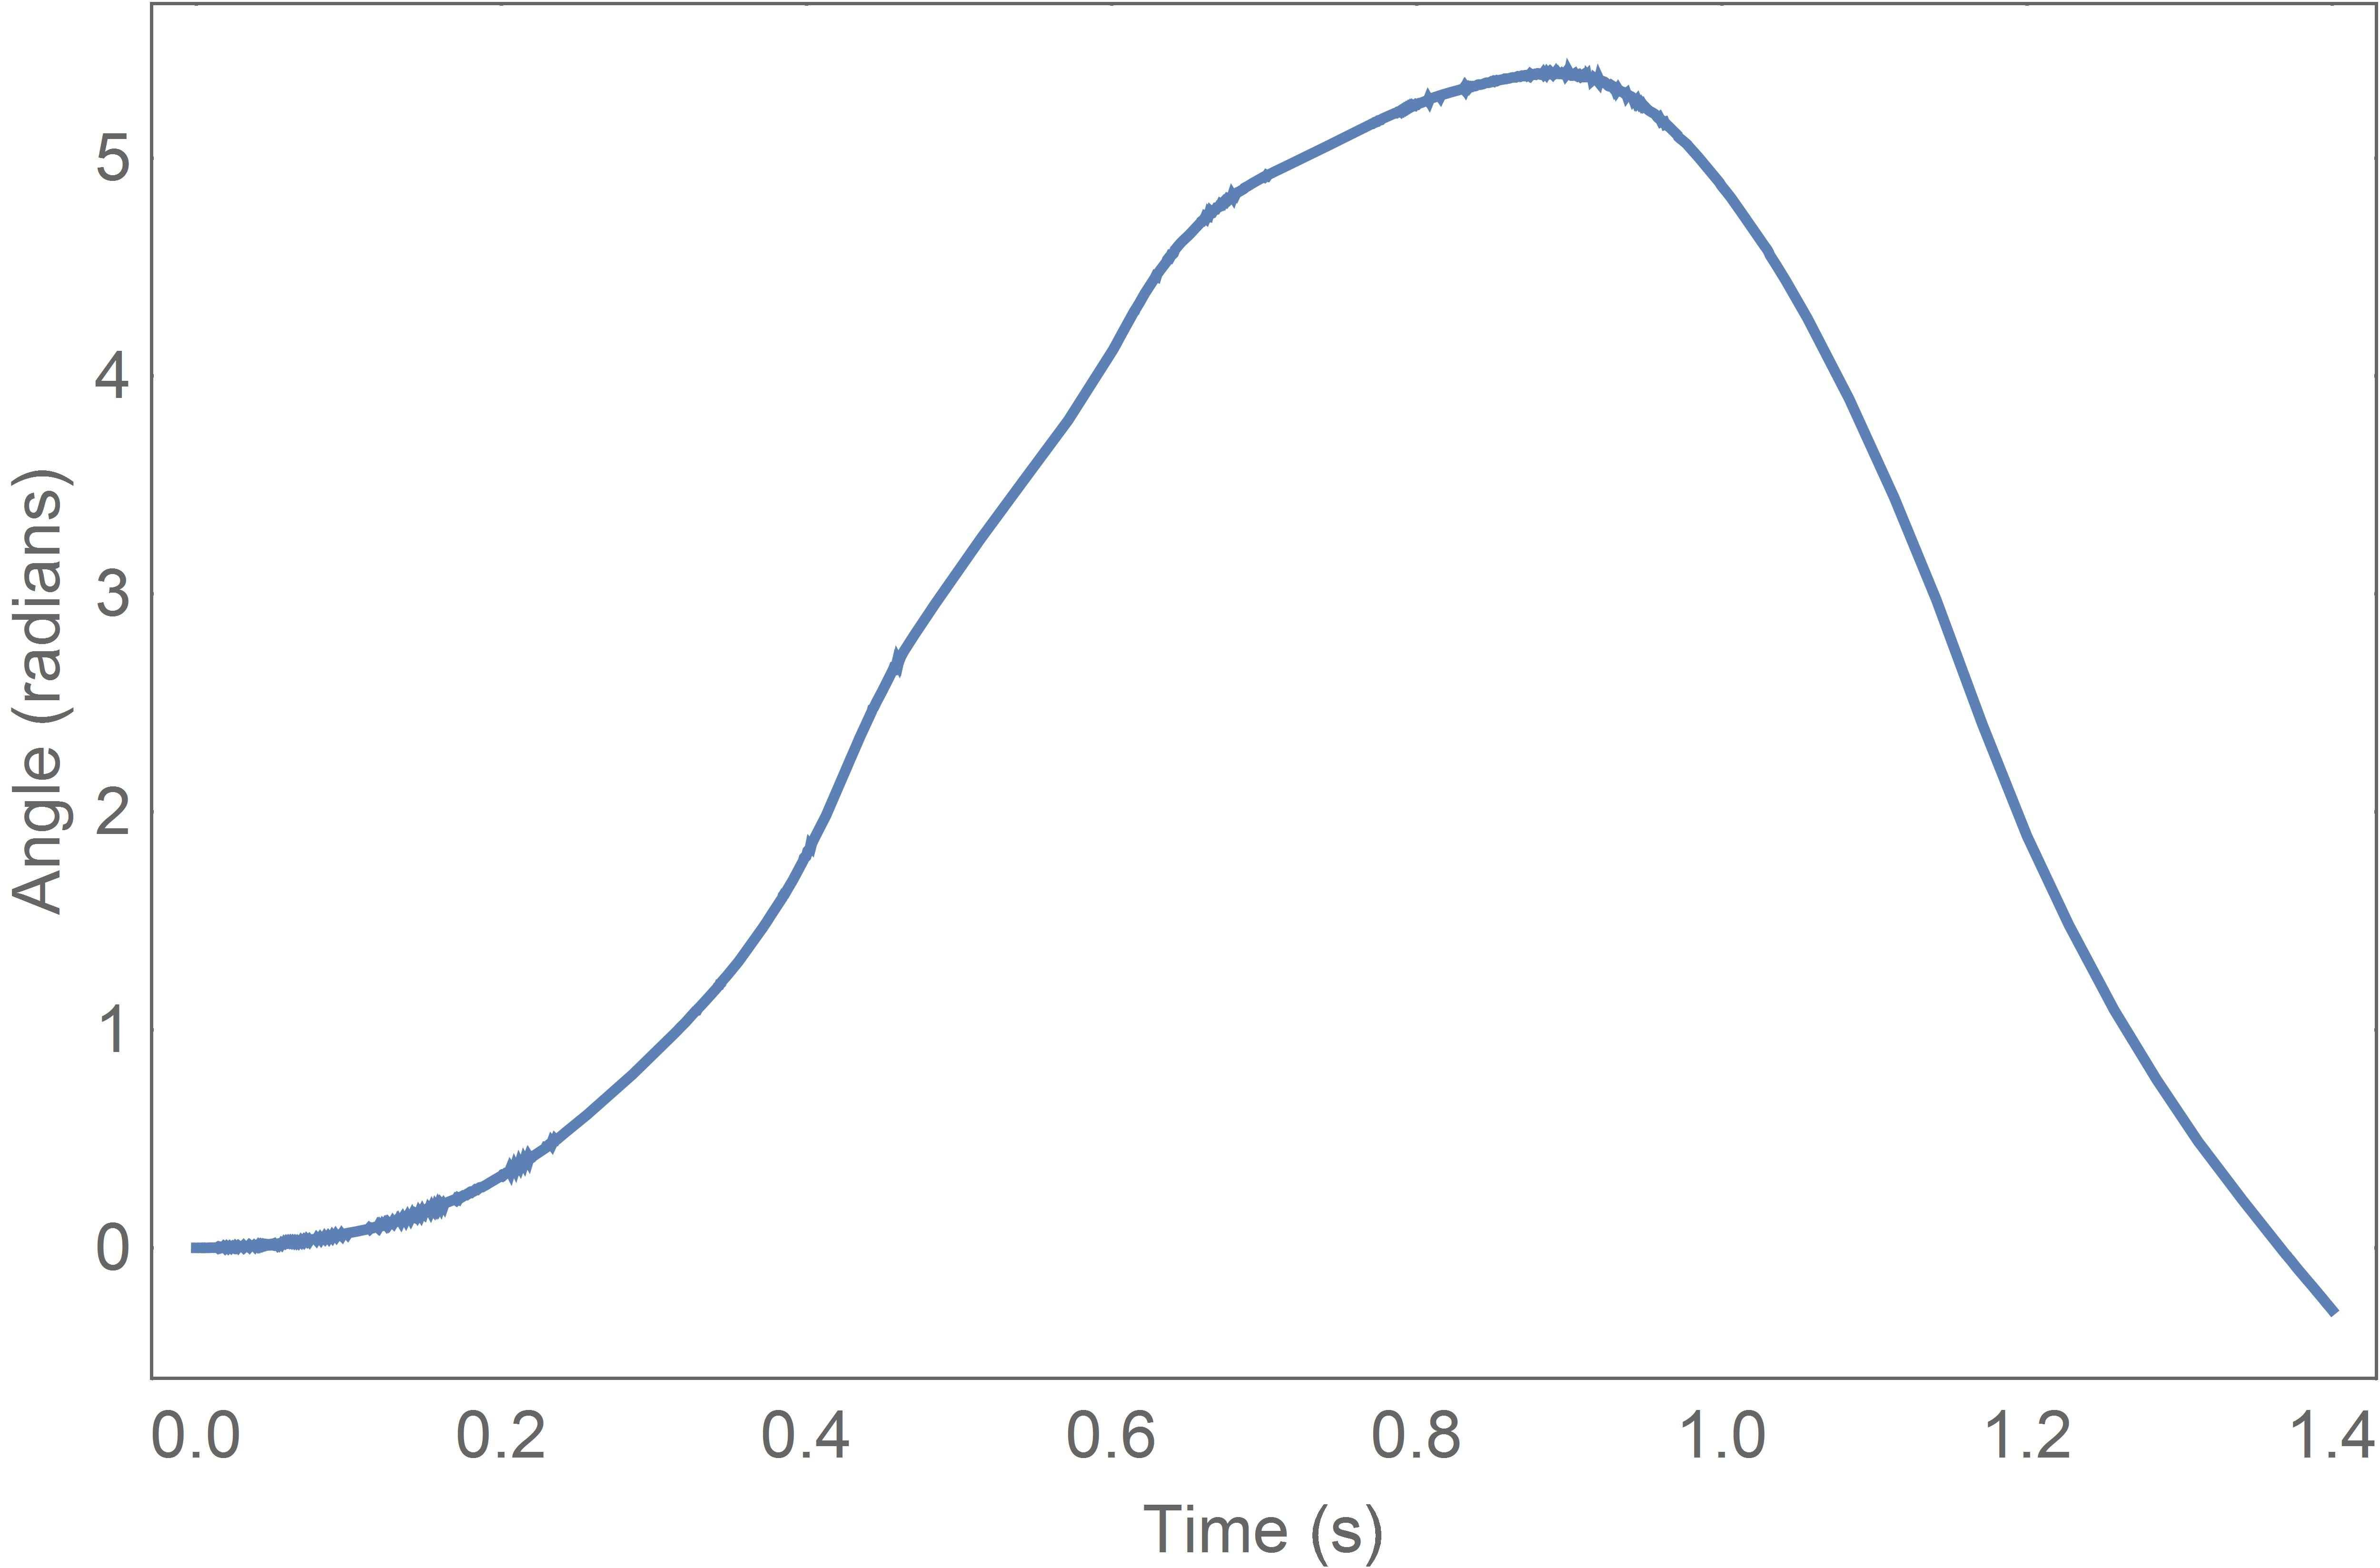
\includegraphics[width=\linewidth]{fallalphafp}
	\endminipage\hspace{1em}%
	\minipage{0.4\textwidth}
	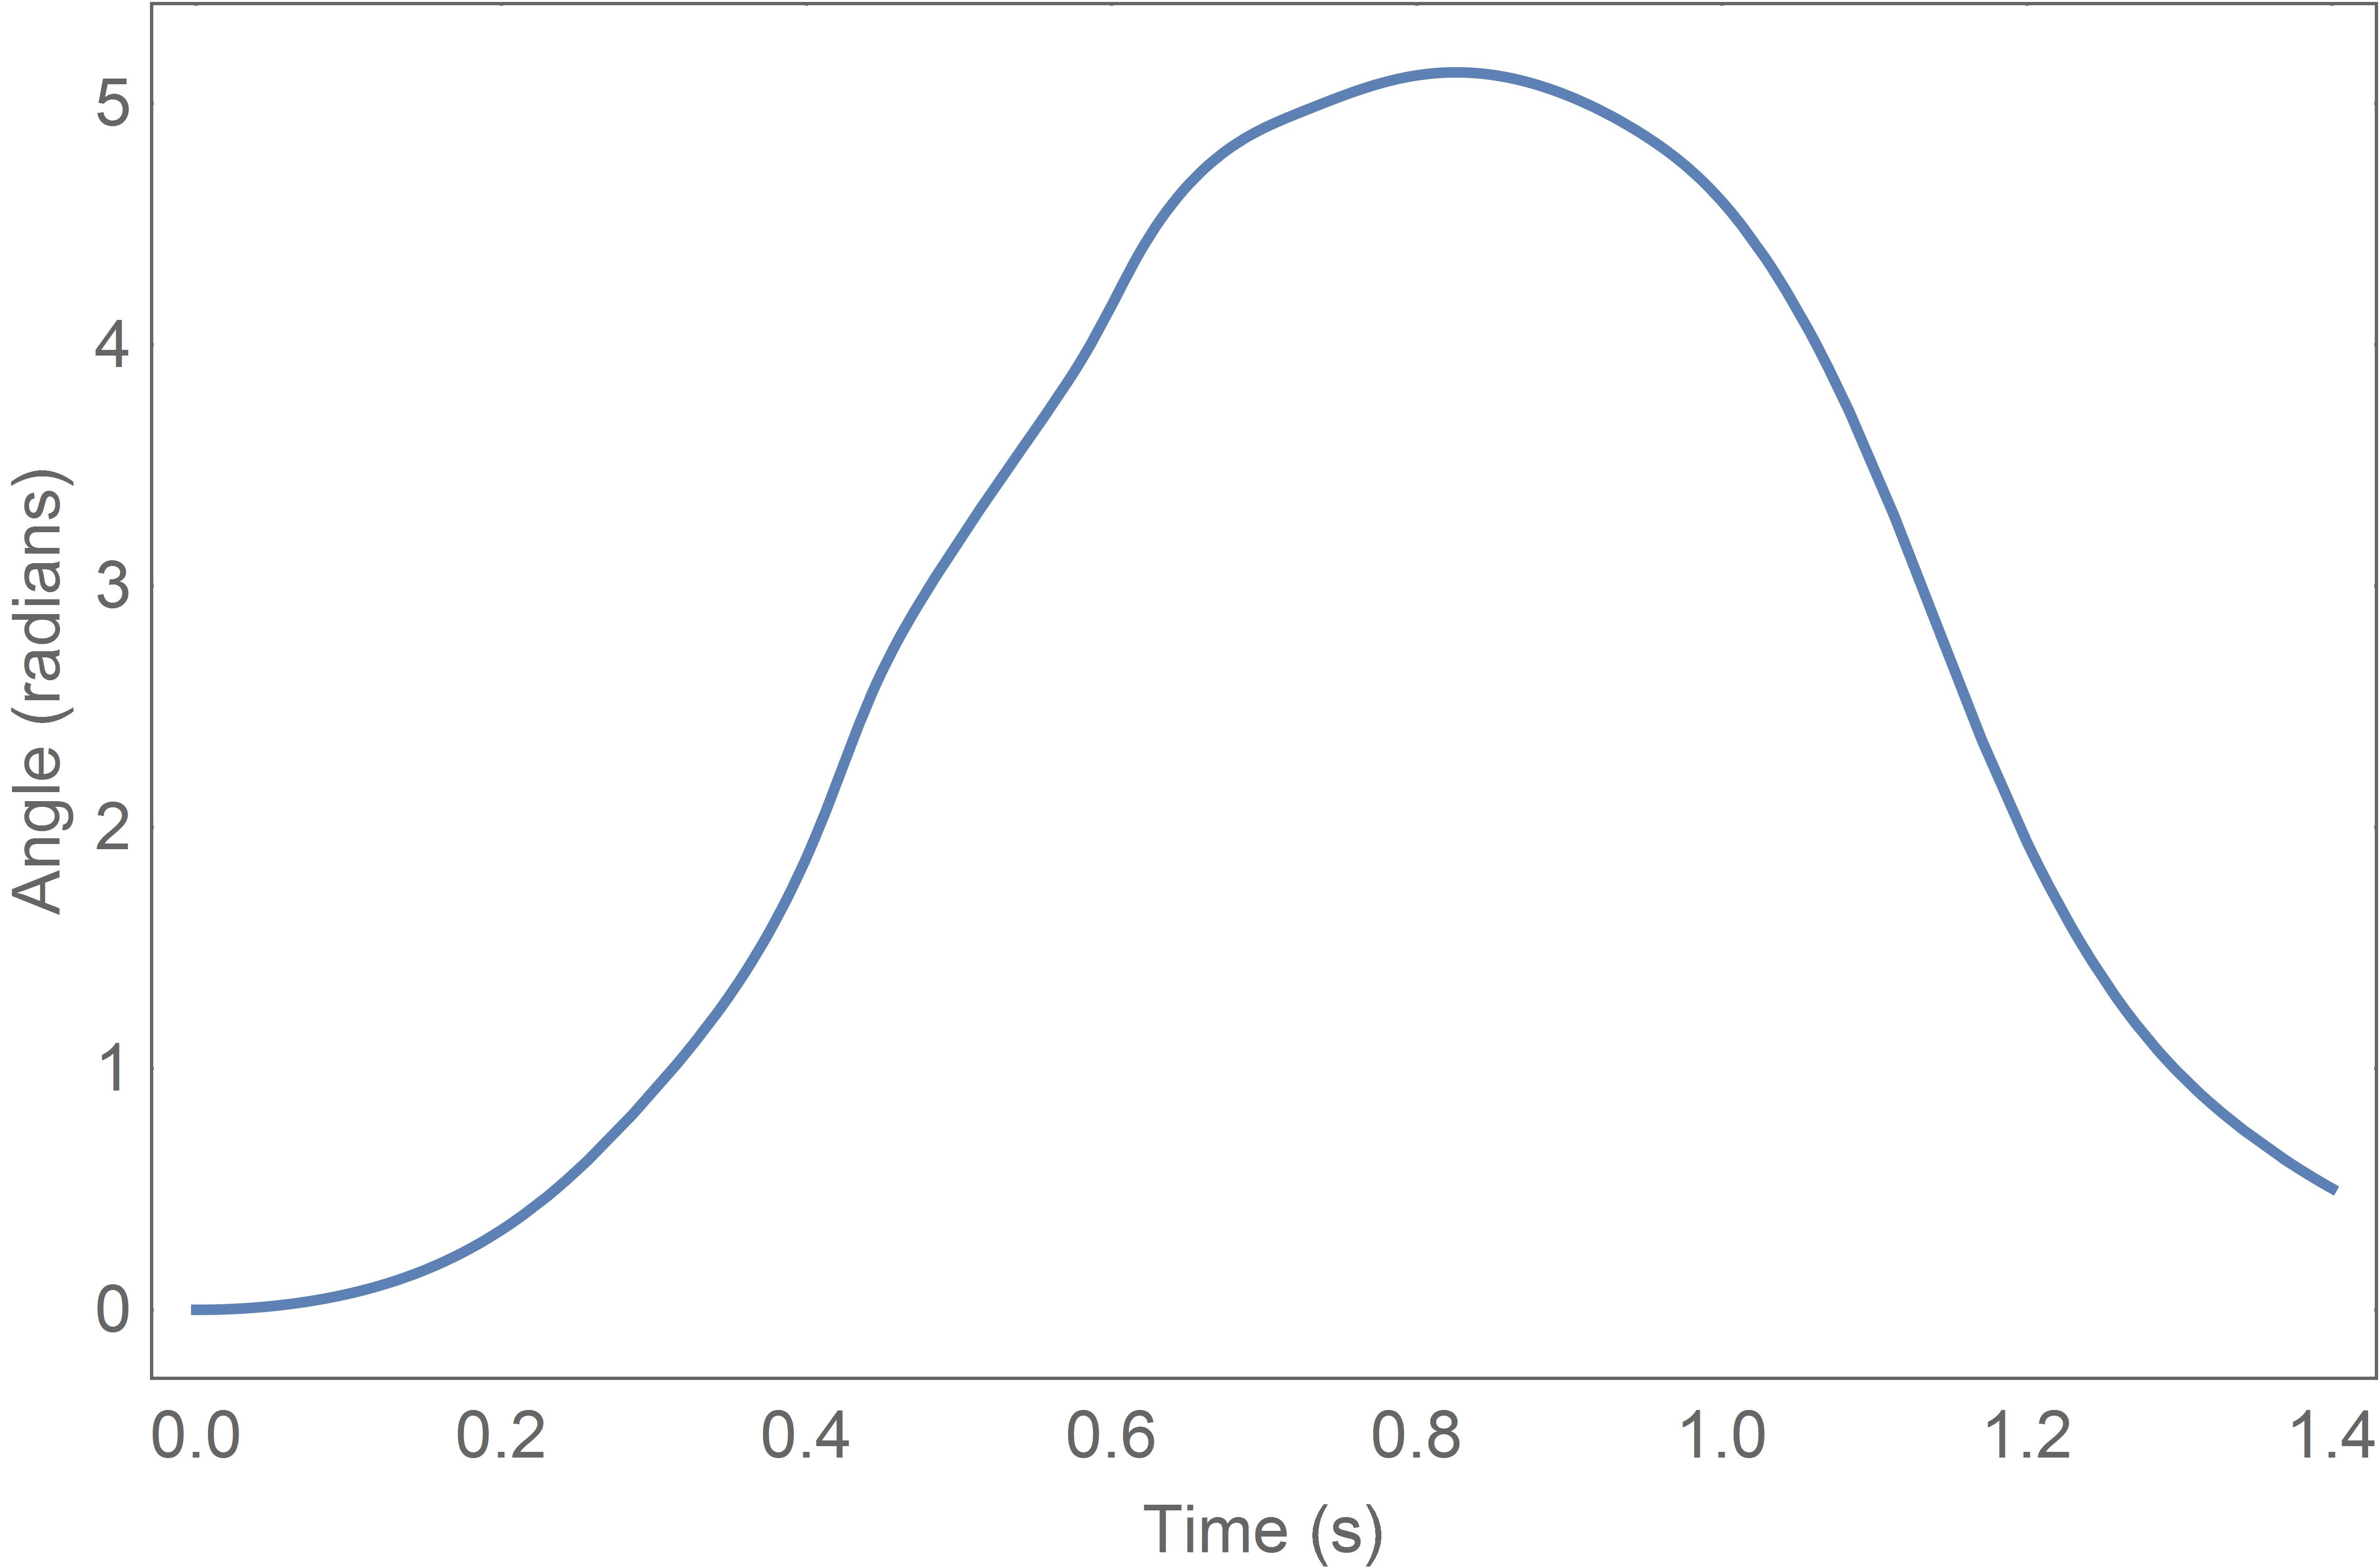
\includegraphics[width=\linewidth]{fallalphabp}
	\endminipage
	\caption{Roll of front plate ($\alpha_{fp}$) and back plate ($\alpha_{bp}$) as the RipStik falls}\label{fig:fallplates}
\end{figure}

\begin{figure}[!htb]
	\centering
	\minipage{0.4\textwidth}
	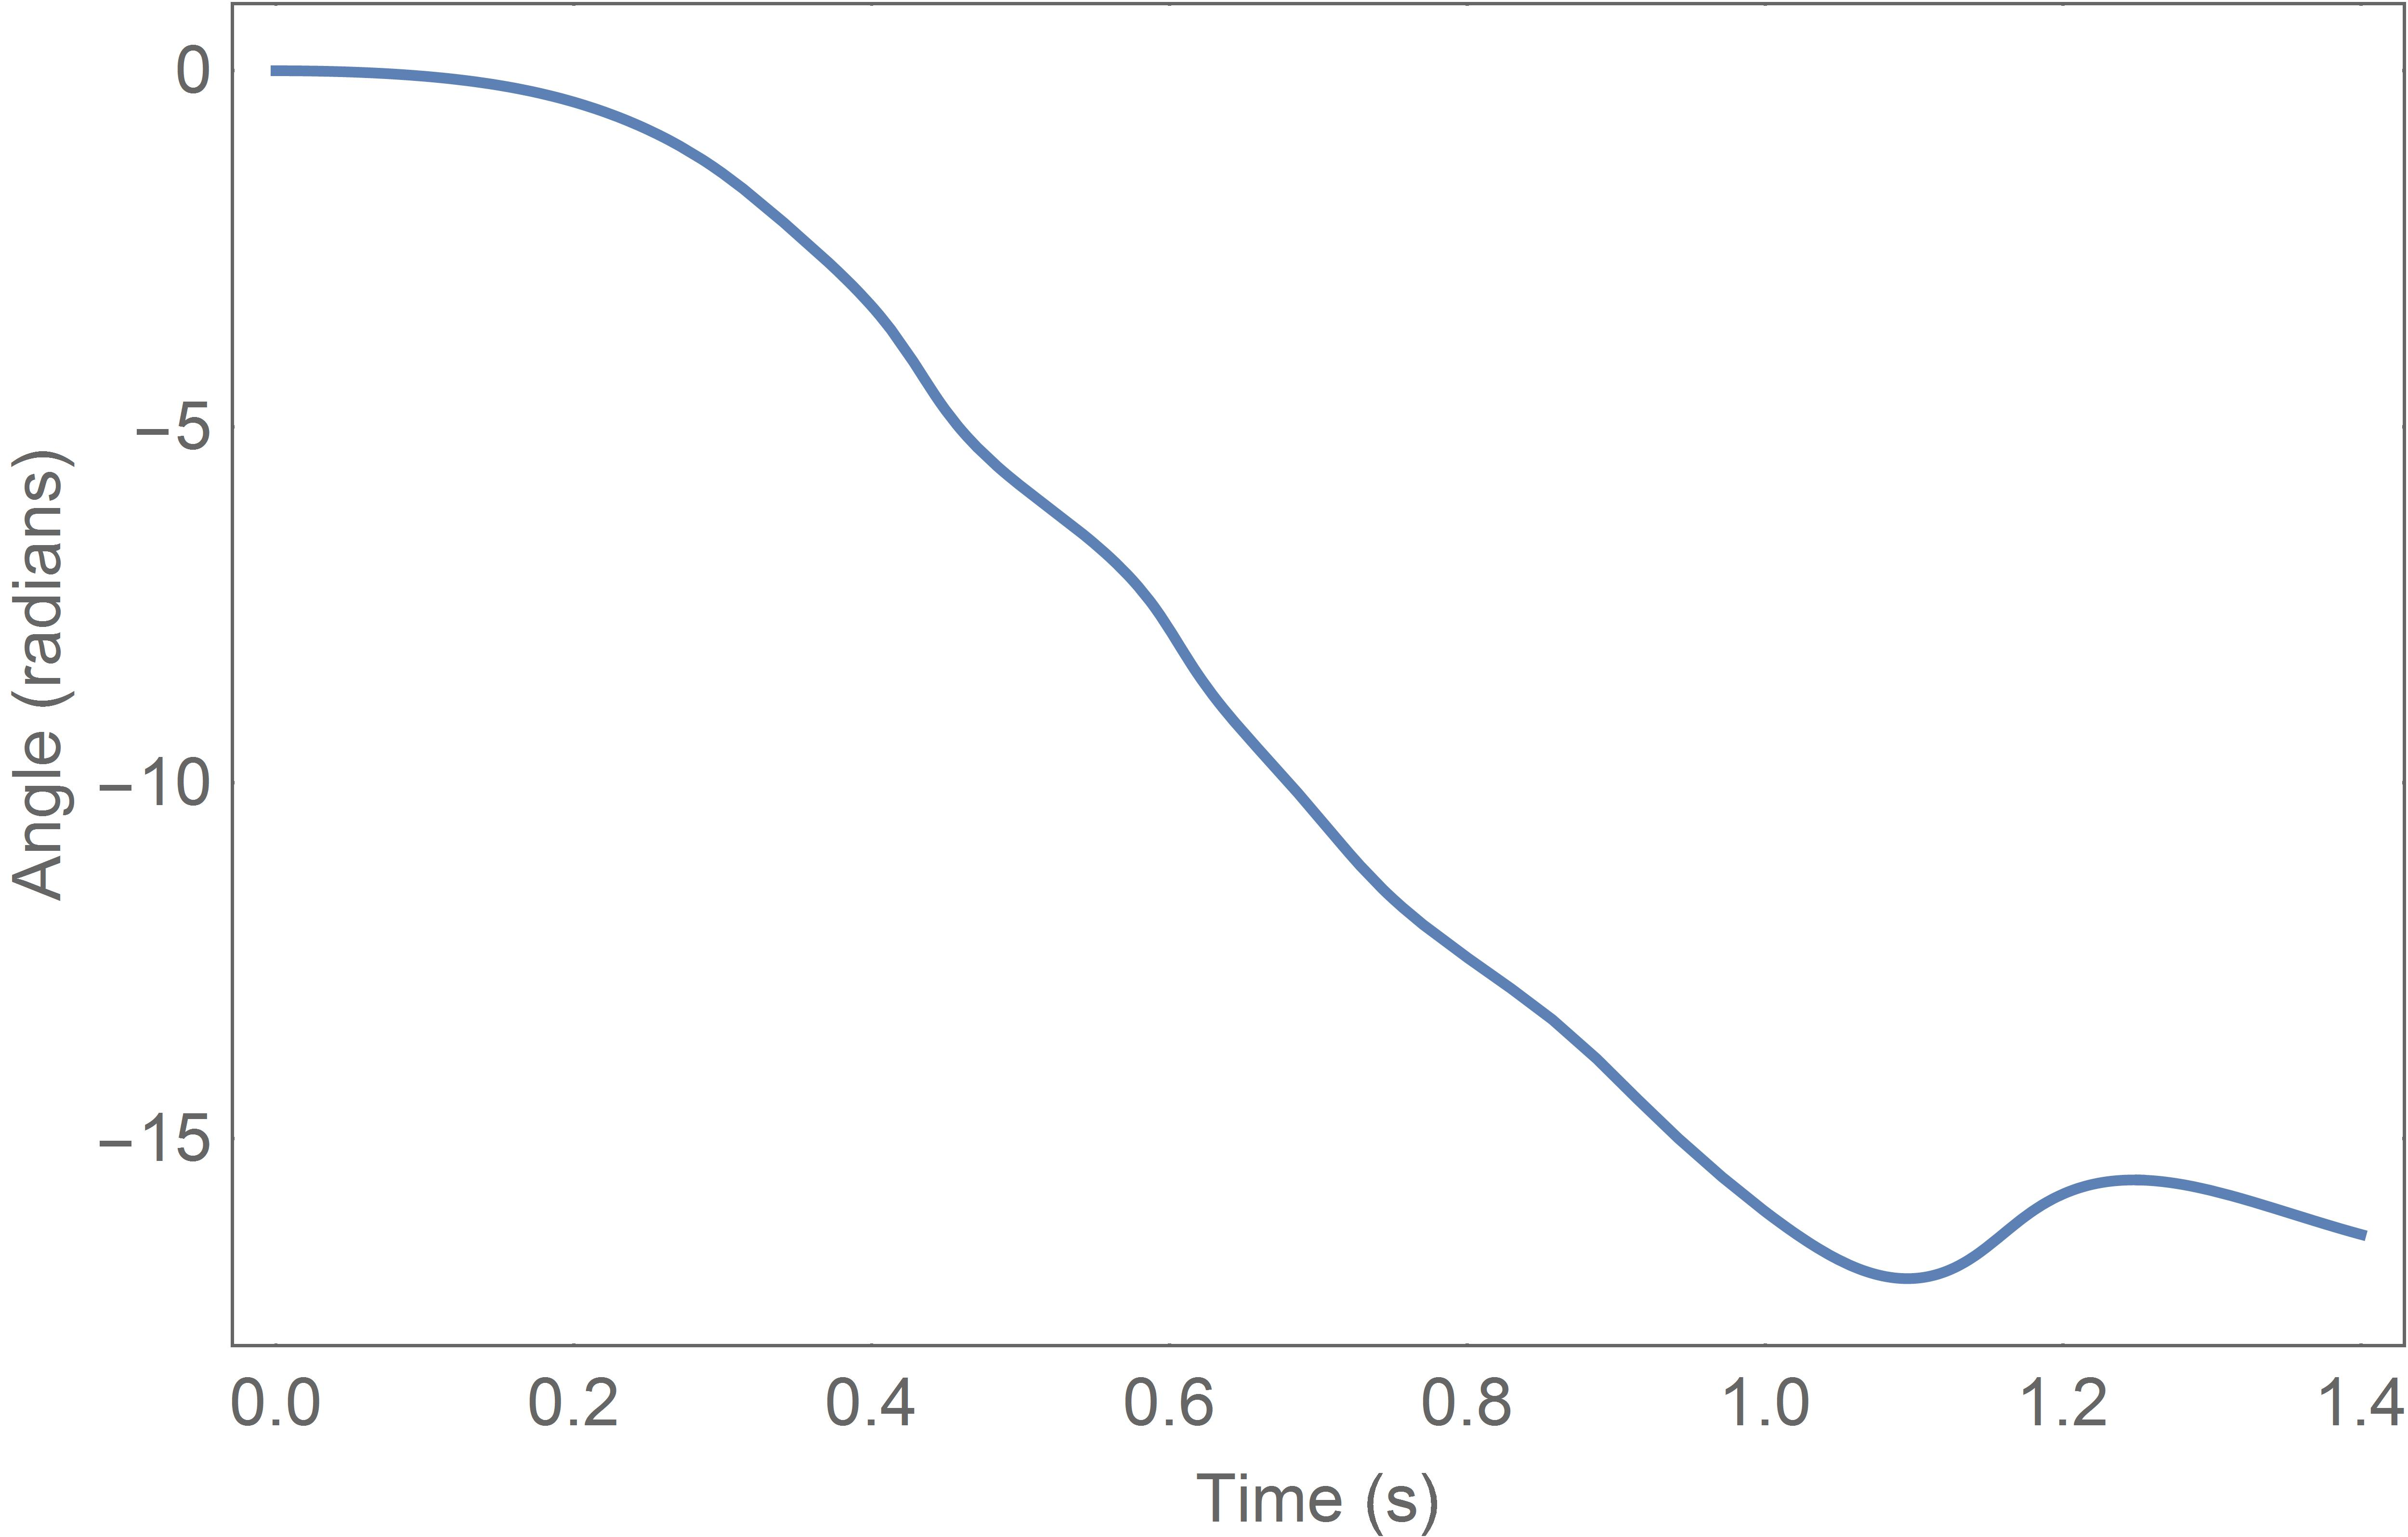
\includegraphics[width=\linewidth]{fallthetafc}
	\endminipage\hspace{1em}%
	\minipage{0.4\textwidth}
	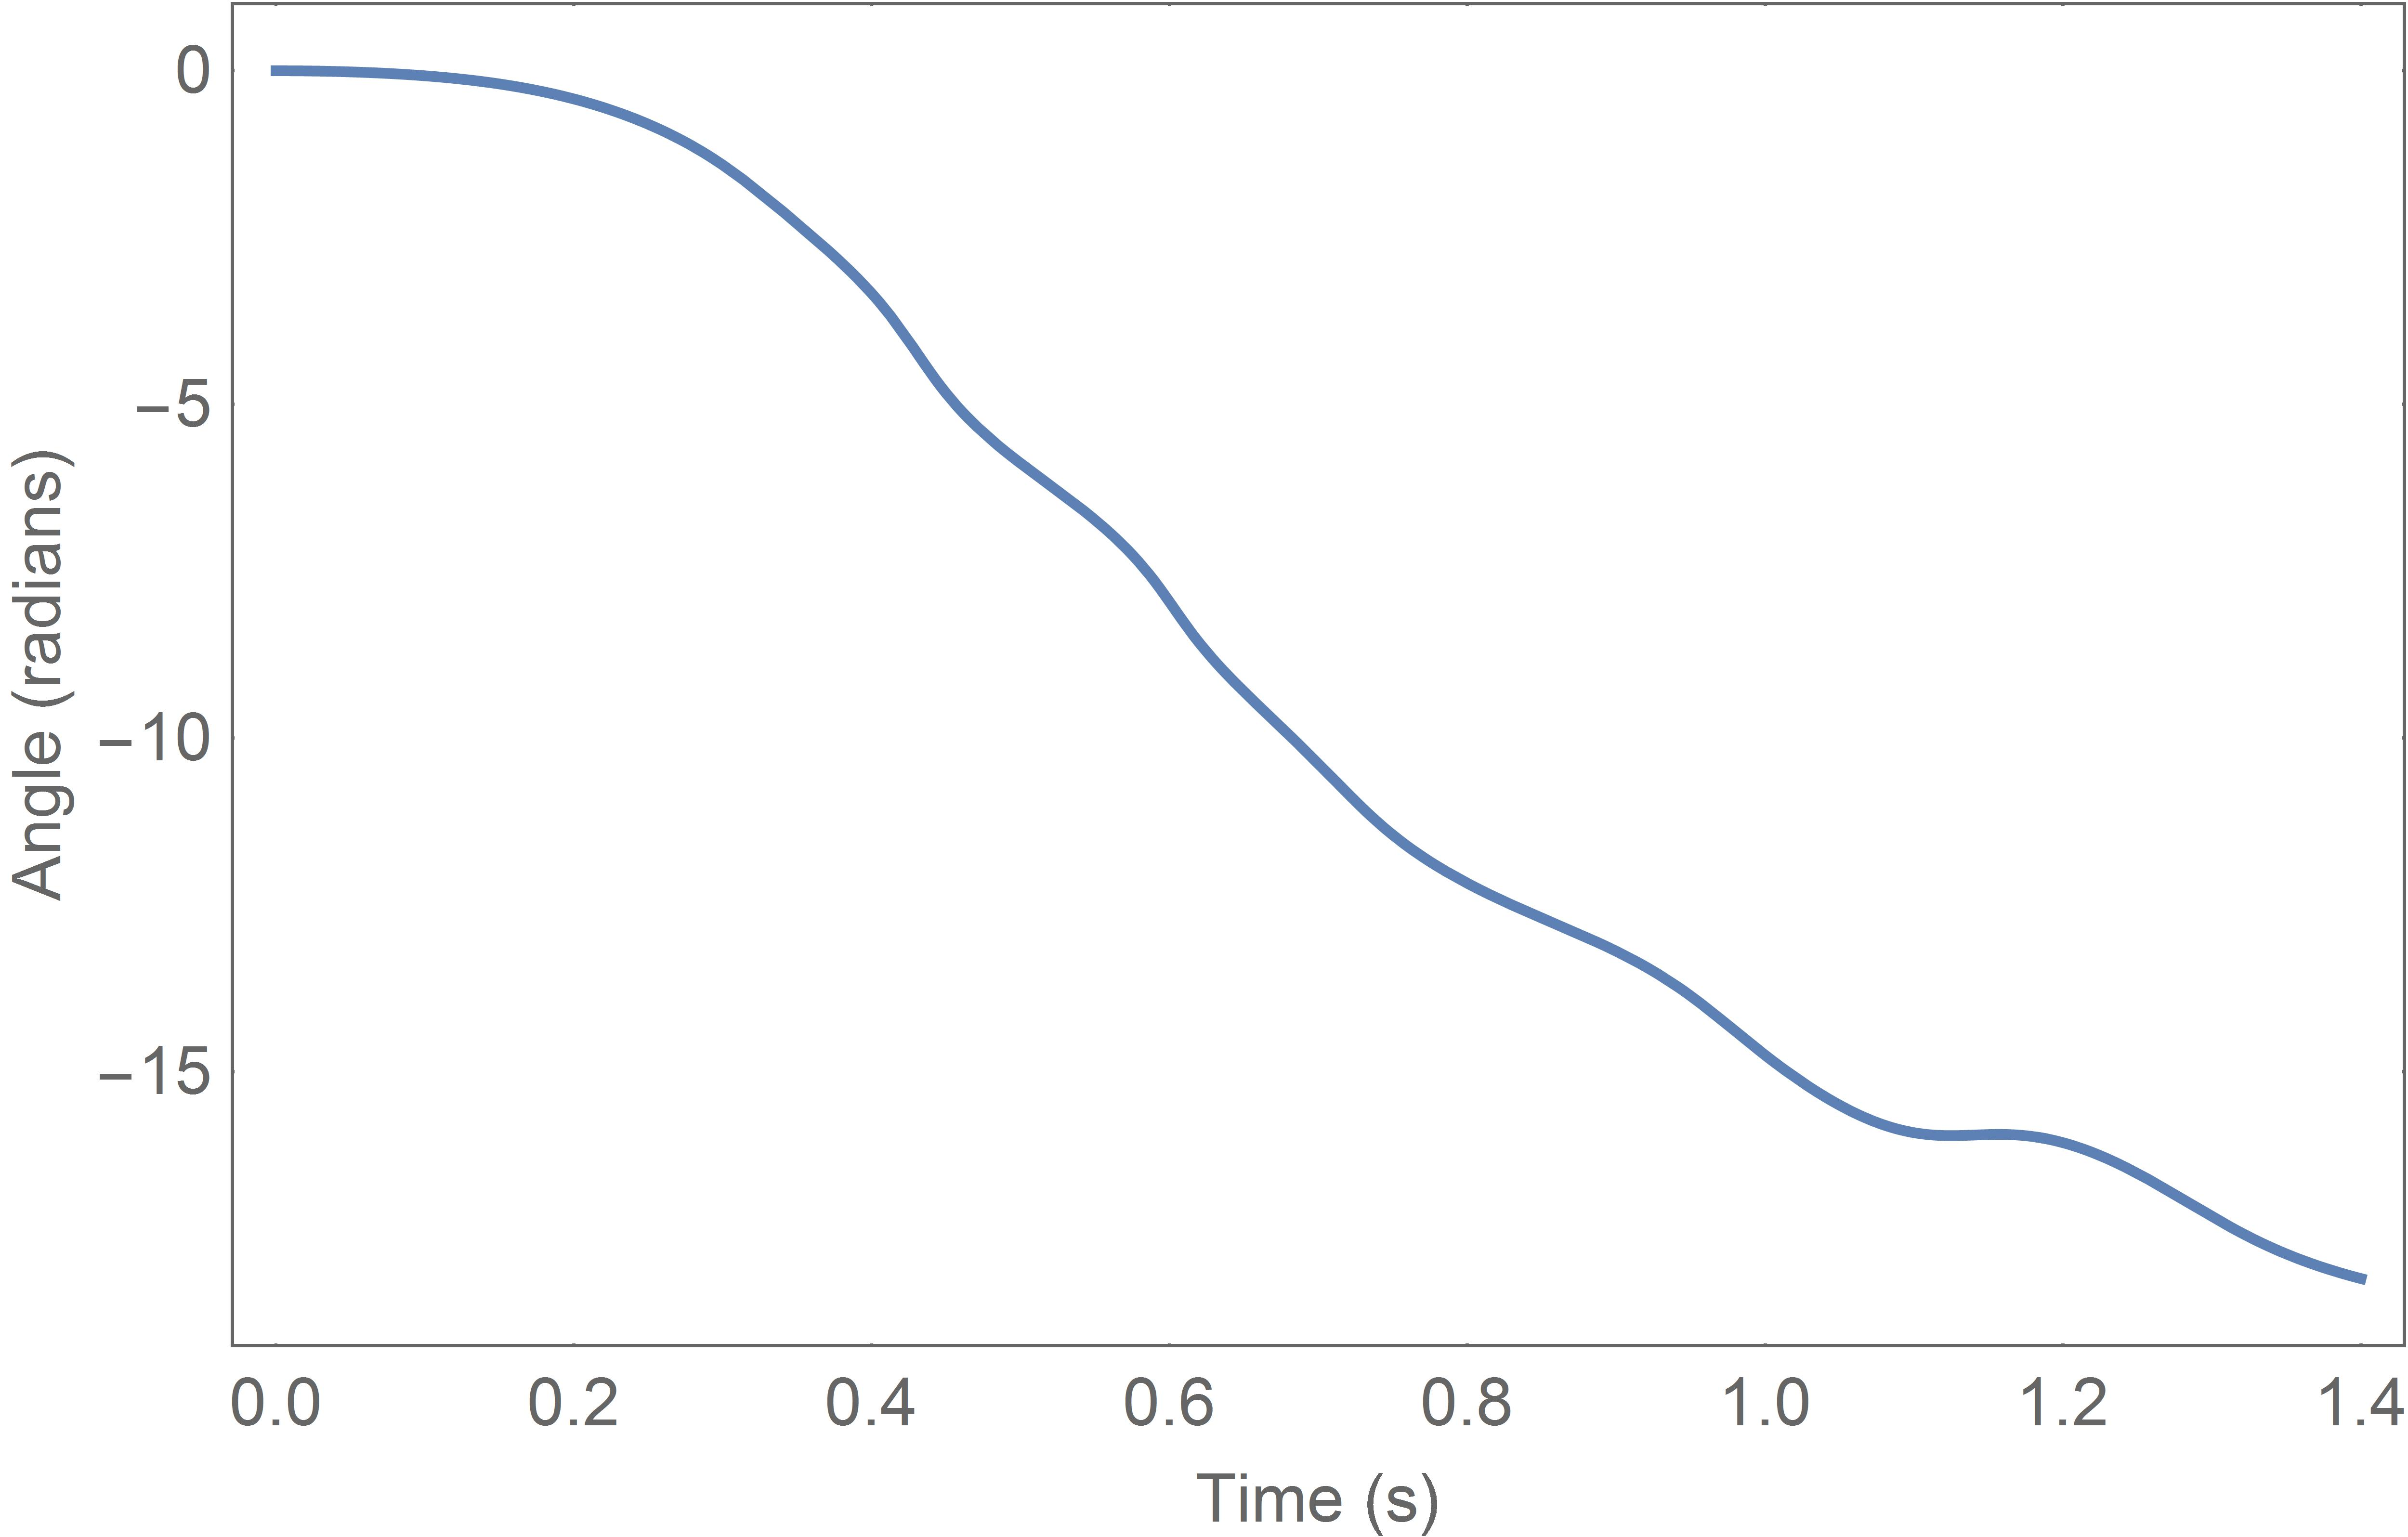
\includegraphics[width=\linewidth]{fallthetabc}
	\endminipage
	\caption{Roll of front caster ($\theta_{fc}$) and back caster ($\theta_{bc}$) as the RipStik falls}\label{fig:fallcaster}	
\end{figure}

The Z-position plot in Figure \ref{fig:fallglobal} shows the Ripstik falling through the ground plane and reorienting itself in the upright position. 
This is clearly illustrated by the oscillations shown in the first plot.


The roll of the front plate ($\alpha_{fp}$) and back plate ($\alpha_{bp}$) plots in Figure \ref{fig:fallplates} show the plates rotating almost 360 degrees, and then rotating fully back to 0. 
This clearly describes the behaviour as the Ripstik essentially flips through the ground plane.
The yaw of the front caster ($\theta_{fc}$) and back caster ($\theta_{bc}$) plots in figure \ref{fig:fallcaster} describe the motion of the casters as the RipStik falls.
The casters pivot to follow the falling motion of the RipStik and satisfy the nonholonomic constraints.
\par
An accurate visualization was produced to model the motion of the RipStik. The initial upright and final fallen over position of the RipStik can be seen in figure

\begin{figure}[!htb]
	\centering
	\minipage{0.4\textwidth}
	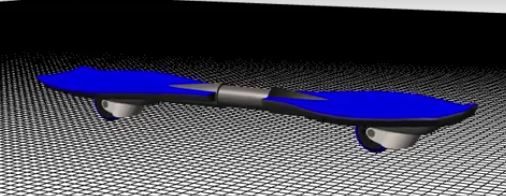
\includegraphics[width=\linewidth]{rest}
	\endminipage\hspace{1em}%
	\minipage{0.37\textwidth}
	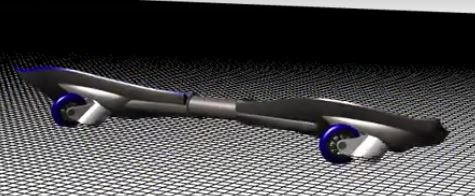
\includegraphics[width=\linewidth]{fall}
	\endminipage
	\caption{Initial upright and final fallen over positions of the RipStik}\label{fig:fallcaster}	
\end{figure}

\subsection{Linear Quadratic Regulator Control}
On the RipStik system, LQR control is intended to be used to stabilize the RipStik about the unstable equilibrium point at the upright position. This means keeping the RipStik platforms stable and level, with the control system forces designed to return the RipStik to this configuration under the effect of external perturbations (i.e. rider instability).

The first concern when implementing LQR control was the effect of the nonholonomic constraints on the linearization process. 
In attempting to solve for the Lagrange multipiers in the linearized equations of motion, two potential methods are considered:
\begin{itemize}
	\item Linearize the system with the unknown constraints to produce a linear DAE then solve for the Lagrange Multipliers
	\item Solve for the Lagrange multipiers then linearize the result
\end{itemize}
In his masters thesis \textit{Linearization and Stability of Nonholonomic Mechanical Systems} \cite{LinNonHolo}, S.D Yang demonstrated a sufficient condition for the commutation of linearizing the equations of motion and solving for Lagrange multipliers. In particular, these operations commute at critical points of the potential function\cite{LinNonHolo}.
The test case developed for LQR control consisted of a rolling wheel (as shown in section \ref{sec:testcaserw}) with an inverted pendulum attached (similar to what was shown in \ref{sec:testcaseip}). Since both components of the mechanical system have been previously developed and validated, minimal additional work is needed to develop the combined system. The system and associated dimensions are shown in \textbf{FIGURE FIGURE}.
The next steps require validating the result discussed from the thesis.

\subsubsection{Test Case - Rolling Wheel with Inverted Pendulum}

\textbf{INSERT FIGURE WITH ANGLES AND JUNK HERE}

Since it was developed in 2 dimensions, the system has 3 degrees of freedom; the horizontal position $x$, the roll angle $\phi$, and the pendulum angle $\psi$. Additionally, the following constants are defined: $m$, the mass of the wheel, $m_p$, the mass of the pendulum, $g$, the acceleration due to gravity, $\rho$, the radius of the wheel, and $L$, the length of the pendulum. Note that the pendulum is again modeled as a thin uniform rod.
The moment of inertia of the wheel is defined to be
\begin{equation}
I_w =
	\begin{pmatrix}
		J_{spin} & 0 & 0 \\
		0 & J_{spin} & 0 \\
		0 & 0 & J_{roll}
	\end{pmatrix},
\end{equation}
for consistency with section \ref{sec:testcaserw}. The rod then has a moment of inertia of \textbf{DO WE NEED A SOURCE ON THIS??}
\begin{equation}
I_p =
	\begin{pmatrix}
		\frac{1}{3}L^{2}m_p & 0 & 0 \\
		0 & \frac{1}{3}L^{2}m_p & 0 \\
		0 & 0 & 0
	\end{pmatrix}.
\end{equation}
The unconstrained Lagrangian of the system is computed to be 
\begin{equation}
\underbrace{m_P \left( g L \sin (\psi (t))- 
	g \rho + 
	\frac{2}{3}L^2 \psi '(t)^2 - 
	L \psi '(t) \sin (\psi (t)) x'(t)+
	\frac{1}{2} x'(t)^2\right)}_{\text{pendulum}} +
	\underbrace{\frac{1}{2} \left(J_{spin} \phi '(t)^2 + 
	m x'(t)^2\right)}_{\text{wheel}} = 0.
\end{equation}
Applying the Euler-Lagrange equation, the unconstrained equations of motion for the system are computed to be 
\begin{equation}
L m_{P} \psi ''(t) \sin (\psi (t))+L m_{P} \psi
   '(t)^2 \cos (\psi (t))-(m+m_{P}) X''(t)=0
\end{equation}
\begin{equation}
   -J_{spin} \phi''(t)=0
\end{equation}
\begin{equation}
   \frac{1}{3} L m_{P} \left(3 g \cos (\psi (t))-4 L \psi ''(t)+3 \sin (\psi (t)) X''(t)\right)=0
\end{equation}
Additionally, system has one nonholonomic constraint, expressed as
\begin{equation}
x'(t) = \rho\theta'(t).
\end{equation}
A control input $f(t)$ was then added to the second equation of motion, thereby applying a torque to the roll angle of the wheel.

In order to experimentally validate the presented result on commutation of linearization and solving for nonholonomic constraints, both procedures were applied to the system. They produced the equivalent linear system
\begin{equation}
\left\{\frac{\left(4 \text{Jspin}+\rho ^2 (4 m+\text{mP})\right)
   \left(L \text{mP} \psi ''(t)+(m+\text{mP}) X''(t)\right)-\rho 
   f(t) (4 m+\text{mP})}{4 \text{Jspin}+\rho ^2 (4
   m+\text{mP})}=0,\frac{\text{Jspin} \left(\phi ''(t) \left(4
   \text{Jspin}+\rho ^2 (4 m+\text{mP})\right)-4 f(t)\right)}{4
   \text{Jspin}+\rho ^2 (4 m+\text{mP})}=0,L \text{mP} \left(4 L
   \psi ''(t)+3 X''(t)\right)=0\right\}
\end{equation}
\subsubsection{Model Implementation Challenges}
\subsubsection{Proposed Testing Framework}


